\documentclass[twoside]{book}

% Packages required by doxygen
\usepackage{fixltx2e}
\usepackage{calc}
\usepackage{doxygen}
\usepackage[export]{adjustbox} % also loads graphicx
\usepackage{graphicx}
\usepackage[utf8]{inputenc}
\usepackage{makeidx}
\usepackage{multicol}
\usepackage{multirow}
\PassOptionsToPackage{warn}{textcomp}
\usepackage{textcomp}
\usepackage[nointegrals]{wasysym}
\usepackage[table]{xcolor}

% Font selection
\usepackage[T1]{fontenc}
\usepackage[scaled=.90]{helvet}
\usepackage{courier}
\usepackage{amssymb}
\usepackage{sectsty}
\renewcommand{\familydefault}{\sfdefault}
\allsectionsfont{%
  \fontseries{bc}\selectfont%
  \color{darkgray}%
}
\renewcommand{\DoxyLabelFont}{%
  \fontseries{bc}\selectfont%
  \color{darkgray}%
}
\newcommand{\+}{\discretionary{\mbox{\scriptsize$\hookleftarrow$}}{}{}}

% Page & text layout
\usepackage{geometry}
\geometry{%
  a4paper,%
  top=2.5cm,%
  bottom=2.5cm,%
  left=2.5cm,%
  right=2.5cm%
}
\tolerance=750
\hfuzz=15pt
\hbadness=750
\setlength{\emergencystretch}{15pt}
\setlength{\parindent}{0cm}
\setlength{\parskip}{3ex plus 2ex minus 2ex}
\makeatletter
\renewcommand{\paragraph}{%
  \@startsection{paragraph}{4}{0ex}{-1.0ex}{1.0ex}{%
    \normalfont\normalsize\bfseries\SS@parafont%
  }%
}
\renewcommand{\subparagraph}{%
  \@startsection{subparagraph}{5}{0ex}{-1.0ex}{1.0ex}{%
    \normalfont\normalsize\bfseries\SS@subparafont%
  }%
}
\makeatother

% Headers & footers
\usepackage{fancyhdr}
\pagestyle{fancyplain}
\fancyhead[LE]{\fancyplain{}{\bfseries\thepage}}
\fancyhead[CE]{\fancyplain{}{}}
\fancyhead[RE]{\fancyplain{}{\bfseries\leftmark}}
\fancyhead[LO]{\fancyplain{}{\bfseries\rightmark}}
\fancyhead[CO]{\fancyplain{}{}}
\fancyhead[RO]{\fancyplain{}{\bfseries\thepage}}
\fancyfoot[LE]{\fancyplain{}{}}
\fancyfoot[CE]{\fancyplain{}{}}
\fancyfoot[RE]{\fancyplain{}{\bfseries\scriptsize Generated by Doxygen }}
\fancyfoot[LO]{\fancyplain{}{\bfseries\scriptsize Generated by Doxygen }}
\fancyfoot[CO]{\fancyplain{}{}}
\fancyfoot[RO]{\fancyplain{}{}}
\renewcommand{\footrulewidth}{0.4pt}
\renewcommand{\chaptermark}[1]{%
  \markboth{#1}{}%
}
\renewcommand{\sectionmark}[1]{%
  \markright{\thesection\ #1}%
}

% Indices & bibliography
\usepackage{natbib}
\usepackage[titles]{tocloft}
\setcounter{tocdepth}{3}
\setcounter{secnumdepth}{5}
\makeindex

% Hyperlinks (required, but should be loaded last)
\usepackage{ifpdf}
\ifpdf
  \usepackage[pdftex,pagebackref=true]{hyperref}
\else
  \usepackage[ps2pdf,pagebackref=true]{hyperref}
\fi
\hypersetup{%
  colorlinks=true,%
  linkcolor=blue,%
  citecolor=blue,%
  unicode%
}

% Custom commands
\newcommand{\clearemptydoublepage}{%
  \newpage{\pagestyle{empty}\cleardoublepage}%
}

\usepackage{caption}
\captionsetup{labelsep=space,justification=centering,font={bf},singlelinecheck=off,skip=4pt,position=top}

%===== C O N T E N T S =====

\begin{document}

% Titlepage & ToC
\hypersetup{pageanchor=false,
             bookmarksnumbered=true,
             pdfencoding=unicode
            }
\pagenumbering{alph}
\begin{titlepage}
\vspace*{7cm}
\begin{center}%
{\Large Beer Game }\\
\vspace*{1cm}
{\large Generated by Doxygen 1.8.13}\\
\end{center}
\end{titlepage}
\clearemptydoublepage
\pagenumbering{roman}
\tableofcontents
\clearemptydoublepage
\pagenumbering{arabic}
\hypersetup{pageanchor=true}

%--- Begin generated contents ---
\chapter{Hierarchical Index}
\section{Class Hierarchy}
This inheritance list is sorted roughly, but not completely, alphabetically\+:\begin{DoxyCompactList}
\item \contentsline{section}{Game}{\pageref{classGame}}{}
\item \contentsline{section}{Instructor}{\pageref{classInstructor}}{}
\item \contentsline{section}{Player}{\pageref{classPlayer}}{}
\item \contentsline{section}{Player\+Event}{\pageref{classPlayerEvent}}{}
\begin{DoxyCompactList}
\item \contentsline{section}{Order}{\pageref{classOrder}}{}
\item \contentsline{section}{Shipment}{\pageref{classShipment}}{}
\end{DoxyCompactList}
\item Q\+Dialog\begin{DoxyCompactList}
\item \contentsline{section}{creategamedialog}{\pageref{classcreategamedialog}}{}
\item \contentsline{section}{currentgamesdialog}{\pageref{classcurrentgamesdialog}}{}
\item \contentsline{section}{player\+Dialog}{\pageref{classplayerDialog}}{}
\item \contentsline{section}{Sec\+Dialog}{\pageref{classSecDialog}}{}
\end{DoxyCompactList}
\item Q\+Main\+Window\begin{DoxyCompactList}
\item \contentsline{section}{Main\+Window}{\pageref{classMainWindow}}{}
\end{DoxyCompactList}
\end{DoxyCompactList}

\chapter{Class Index}
\section{Class List}
Here are the classes, structs, unions and interfaces with brief descriptions\+:\begin{DoxyCompactList}
\item\contentsline{section}{\hyperlink{classcreategamedialog}{creategamedialog} }{\pageref{classcreategamedialog}}{}
\item\contentsline{section}{\hyperlink{classcurrentgamesdialog}{currentgamesdialog} }{\pageref{classcurrentgamesdialog}}{}
\item\contentsline{section}{\hyperlink{classGame}{Game} \\*The \hyperlink{classGame}{Game} class }{\pageref{classGame}}{}
\item\contentsline{section}{\hyperlink{classInstructor}{Instructor} \\*The \hyperlink{classInstructor}{Instructor} class }{\pageref{classInstructor}}{}
\item\contentsline{section}{\hyperlink{classMainWindow}{Main\+Window} }{\pageref{classMainWindow}}{}
\item\contentsline{section}{\hyperlink{classOrder}{Order} \\*The \hyperlink{classOrder}{Order} class }{\pageref{classOrder}}{}
\item\contentsline{section}{\hyperlink{classPlayer}{Player} \\*The \hyperlink{classPlayer}{Player} class }{\pageref{classPlayer}}{}
\item\contentsline{section}{\hyperlink{classplayerDialog}{player\+Dialog} }{\pageref{classplayerDialog}}{}
\item\contentsline{section}{\hyperlink{classPlayerEvent}{Player\+Event} \\*The \hyperlink{classPlayerEvent}{Player\+Event} class }{\pageref{classPlayerEvent}}{}
\item\contentsline{section}{\hyperlink{classSecDialog}{Sec\+Dialog} }{\pageref{classSecDialog}}{}
\item\contentsline{section}{\hyperlink{classShipment}{Shipment} \\*The \hyperlink{classShipment}{Shipment} class }{\pageref{classShipment}}{}
\end{DoxyCompactList}

\chapter{File Index}
\doxysection{File List}
Here is a list of all files with brief descriptions\+:\begin{DoxyCompactList}
\item\contentsline{section}{/home/diggy/sprint-\/1/src/\mbox{\hyperlink{factory_8cpp}{factory.\+cpp}} }{\pageref{factory_8cpp}}{}
\item\contentsline{section}{/home/diggy/sprint-\/1/src/\mbox{\hyperlink{factory_8h}{factory.\+h}} }{\pageref{factory_8h}}{}
\item\contentsline{section}{/home/diggy/sprint-\/1/src/\mbox{\hyperlink{game_8cpp}{game.\+cpp}} }{\pageref{game_8cpp}}{}
\item\contentsline{section}{/home/diggy/sprint-\/1/src/\mbox{\hyperlink{game_8h}{game.\+h}} }{\pageref{game_8h}}{}
\item\contentsline{section}{/home/diggy/sprint-\/1/src/\mbox{\hyperlink{instructor_8cpp}{instructor.\+cpp}} }{\pageref{instructor_8cpp}}{}
\item\contentsline{section}{/home/diggy/sprint-\/1/src/\mbox{\hyperlink{instructor_8h}{instructor.\+h}} }{\pageref{instructor_8h}}{}
\item\contentsline{section}{/home/diggy/sprint-\/1/src/\mbox{\hyperlink{main_8cpp}{main.\+cpp}} }{\pageref{main_8cpp}}{}
\item\contentsline{section}{/home/diggy/sprint-\/1/src/\mbox{\hyperlink{mainwindow_8cpp}{mainwindow.\+cpp}} }{\pageref{mainwindow_8cpp}}{}
\item\contentsline{section}{/home/diggy/sprint-\/1/src/\mbox{\hyperlink{mainwindow_8h}{mainwindow.\+h}} }{\pageref{mainwindow_8h}}{}
\item\contentsline{section}{/home/diggy/sprint-\/1/src/\mbox{\hyperlink{order_8cpp}{order.\+cpp}} }{\pageref{order_8cpp}}{}
\item\contentsline{section}{/home/diggy/sprint-\/1/src/\mbox{\hyperlink{order_8h}{order.\+h}} }{\pageref{order_8h}}{}
\item\contentsline{section}{/home/diggy/sprint-\/1/src/\mbox{\hyperlink{player_8cpp}{player.\+cpp}} }{\pageref{player_8cpp}}{}
\item\contentsline{section}{/home/diggy/sprint-\/1/src/\mbox{\hyperlink{player_8h}{player.\+h}} }{\pageref{player_8h}}{}
\end{DoxyCompactList}

\chapter{Class Documentation}
\hypertarget{classcreategamedialog}{}\section{creategamedialog Class Reference}
\label{classcreategamedialog}\index{creategamedialog@{creategamedialog}}


Inheritance diagram for creategamedialog\+:\nopagebreak
\begin{figure}[H]
\begin{center}
\leavevmode
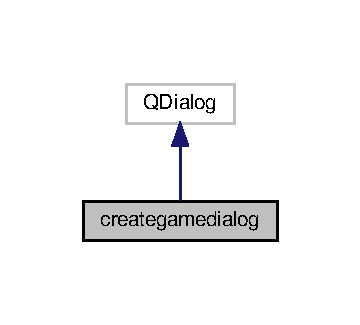
\includegraphics[width=173pt]{classcreategamedialog__inherit__graph}
\end{center}
\end{figure}


Collaboration diagram for creategamedialog\+:\nopagebreak
\begin{figure}[H]
\begin{center}
\leavevmode
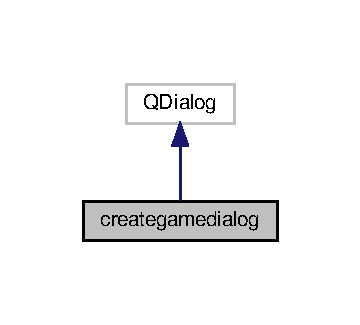
\includegraphics[width=173pt]{classcreategamedialog__coll__graph}
\end{center}
\end{figure}
\subsection*{Public Member Functions}
\begin{DoxyCompactItemize}
\item 
\mbox{\Hypertarget{classcreategamedialog_afb6ad2b9afb5d99b111bc0aeb32fcca6}\label{classcreategamedialog_afb6ad2b9afb5d99b111bc0aeb32fcca6}} 
{\bfseries creategamedialog} (Q\+Widget $\ast$parent=0)
\end{DoxyCompactItemize}


The documentation for this class was generated from the following files\+:\begin{DoxyCompactItemize}
\item 
src/creategamedialog.\+h\item 
src/creategamedialog.\+cpp\end{DoxyCompactItemize}

\hypertarget{classcurrentgamesdialog}{}\section{currentgamesdialog Class Reference}
\label{classcurrentgamesdialog}\index{currentgamesdialog@{currentgamesdialog}}


Inheritance diagram for currentgamesdialog\+:\nopagebreak
\begin{figure}[H]
\begin{center}
\leavevmode
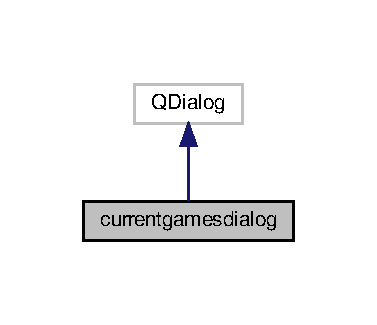
\includegraphics[width=181pt]{classcurrentgamesdialog__inherit__graph}
\end{center}
\end{figure}


Collaboration diagram for currentgamesdialog\+:\nopagebreak
\begin{figure}[H]
\begin{center}
\leavevmode
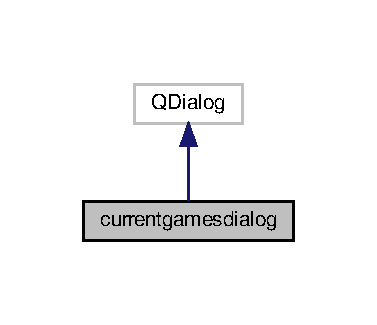
\includegraphics[width=181pt]{classcurrentgamesdialog__coll__graph}
\end{center}
\end{figure}
\subsection*{Public Member Functions}
\begin{DoxyCompactItemize}
\item 
\mbox{\Hypertarget{classcurrentgamesdialog_a51d424ef123e1a040d859ee7fd94f2c3}\label{classcurrentgamesdialog_a51d424ef123e1a040d859ee7fd94f2c3}} 
{\bfseries currentgamesdialog} (Q\+Widget $\ast$parent=0)
\end{DoxyCompactItemize}


The documentation for this class was generated from the following files\+:\begin{DoxyCompactItemize}
\item 
src/currentgamesdialog.\+h\item 
src/currentgamesdialog.\+cpp\end{DoxyCompactItemize}

\hypertarget{classGame}{}\section{Game Class Reference}
\label{classGame}\index{Game@{Game}}


The \hyperlink{classGame}{Game} class.  




{\ttfamily \#include $<$game.\+h$>$}

\subsection*{Public Member Functions}
\begin{DoxyCompactItemize}
\item 
void \hyperlink{classGame_ab3646e6404630076f38d56c1ed36537a}{set\+Number\+Of\+Players} (unsigned int nr)
\begin{DoxyCompactList}\small\item\em Setter Method for number of players. \end{DoxyCompactList}\item 
unsigned int \hyperlink{classGame_a6118afd4e0300b2e855e42fb8400411c}{get\+Number\+Of\+Players} ()
\begin{DoxyCompactList}\small\item\em Getter Method for number of players. \end{DoxyCompactList}\item 
void \hyperlink{classGame_a6b53474fddd090df8ee7eb00512fccb6}{set\+Factory\+Delay} (unsigned int nr)
\begin{DoxyCompactList}\small\item\em Setter Method for factory delay. \end{DoxyCompactList}\item 
unsigned int \hyperlink{classGame_a924b77b7e4e073da9fd634e5200c8358}{get\+Factory\+Delay} ()
\begin{DoxyCompactList}\small\item\em Getter Method for Factory delay. \end{DoxyCompactList}\item 
void \hyperlink{classGame_a5cb92fa59d3d5e06c1b8f4349308b315}{startgame} ()
\begin{DoxyCompactList}\small\item\em Method for Starting game. \end{DoxyCompactList}\item 
void \hyperlink{classGame_a8d55289a3b6f78014ac06f2faa0a7335}{add\+Player} (\hyperlink{classPlayer}{Player} p)
\begin{DoxyCompactList}\small\item\em Method for adding players. \end{DoxyCompactList}\item 
\hyperlink{classPlayer}{Player} $\ast$ \hyperlink{classGame_ac055ae02c6ab4a4f2a6099da86b97932}{get\+Upstream} (int role)
\begin{DoxyCompactList}\small\item\em Getter Method for Upstream. \end{DoxyCompactList}\item 
\hyperlink{classPlayer}{Player} $\ast$ \hyperlink{classGame_afd99959acb65696ddab45bdedf7b17fb}{get\+Downstream} (int role)
\begin{DoxyCompactList}\small\item\em Getter Method for Downstream. \end{DoxyCompactList}\item 
void \hyperlink{classGame_a907d3c04b949ddcf3d528a0c45122ba8}{execute\+Orders\+For\+Current\+Week} ()
\begin{DoxyCompactList}\small\item\em Method for executing orders for current week. \end{DoxyCompactList}\item 
void \hyperlink{classGame_ab3dc5ad2b07ebdab4ed710904bb629e8}{execute\+Shipments\+For\+Current\+Week} ()
\begin{DoxyCompactList}\small\item\em Method for executing shipment for current week. \end{DoxyCompactList}\item 
void \hyperlink{classGame_ac586db141ef21c992a6474300bdea2d0}{update\+Player\+Inventories} ()
\begin{DoxyCompactList}\small\item\em Method for. \end{DoxyCompactList}\item 
int \hyperlink{classGame_a8471ea91ed18fc2d289eb23747d11d39}{advance\+Week} ()
\begin{DoxyCompactList}\small\item\em Method for. \end{DoxyCompactList}\item 
void \hyperlink{classGame_a2cfb2422cb425f254c0cb455fefa0fb5}{add\+Order} (int role, int numberof\+Beers)
\begin{DoxyCompactList}\small\item\em Method for. \end{DoxyCompactList}\item 
void \hyperlink{classGame_a378029f01136b72969cba2cd716ff028}{add\+Shipment} (int role, int numberof\+Beers)
\begin{DoxyCompactList}\small\item\em Method for. \end{DoxyCompactList}\item 
std\+::vector$<$ std\+::string $>$ \hyperlink{classGame_abb451d6df42d5c439e4f3e16627732fd}{generate\+Passwords} ()
\begin{DoxyCompactList}\small\item\em Method for. \end{DoxyCompactList}\item 
unsigned int \hyperlink{classGame_aa4a7ec996cff81f9b7b6e90103ff2a1a}{get\+G\+Id} () const
\begin{DoxyCompactList}\small\item\em Implementation of getters and setter for this class. \end{DoxyCompactList}\item 
void \hyperlink{classGame_ab7b398c385cec5ea920d1b5053a1e707}{set\+G\+Id} (unsigned int value)
\begin{DoxyCompactList}\small\item\em Setter Method for gid. \end{DoxyCompactList}\item 
unsigned int \hyperlink{classGame_acbda63cea0b23cda6e11c4384bf4a869}{get\+Instr\+Id} () const
\begin{DoxyCompactList}\small\item\em Getter Method for the \hyperlink{classInstructor}{Instructor} Id. \end{DoxyCompactList}\item 
void \hyperlink{classGame_a6548484fe42f375e949b52c96a0bc348}{set\+Instr\+Id} (unsigned int value)
\begin{DoxyCompactList}\small\item\em Setter Method for the value of \hyperlink{classInstructor}{Instructor} Id. \end{DoxyCompactList}\item 
unsigned int \hyperlink{classGame_a9e03bc7bd2beb1b5077db5905dbc8146}{get\+P\+Fact\+Id} () const
\begin{DoxyCompactList}\small\item\em Getter Method for factory player id. \end{DoxyCompactList}\item 
void \hyperlink{classGame_a144ffe419003a0cb19001c46109a6bfe}{set\+P\+Fact\+Id} (unsigned int value)
\begin{DoxyCompactList}\small\item\em Setter Method for Factory player id. \end{DoxyCompactList}\item 
unsigned int \hyperlink{classGame_a55ce7f3ec72183e839c3139db478e367}{get\+P\+Distributor\+Id} () const
\begin{DoxyCompactList}\small\item\em Getter Method for distributor player id. \end{DoxyCompactList}\item 
void \hyperlink{classGame_ab88440f7297899b9e534f314f5f49eaa}{set\+P\+Distributor\+Id} (unsigned int value)
\begin{DoxyCompactList}\small\item\em Setter Method for Distributor player id. \end{DoxyCompactList}\item 
unsigned int \hyperlink{classGame_a8197219d0ce49f5ac76d1ed6890cfb3e}{get\+P\+Wholesaler\+Id} () const
\begin{DoxyCompactList}\small\item\em Getter Method for wholesaler player id. \end{DoxyCompactList}\item 
void \hyperlink{classGame_ae192d77627e937d9840f77126fc0b3b7}{set\+P\+Wholesaler\+Id} (unsigned int value)
\begin{DoxyCompactList}\small\item\em Setter Method for. \end{DoxyCompactList}\item 
unsigned int \hyperlink{classGame_a22a98a8e7701f22e9bf5c1c011724154}{get\+Retailer\+Id} () const
\begin{DoxyCompactList}\small\item\em Getter Method for retailer player id. \end{DoxyCompactList}\item 
void \hyperlink{classGame_a676c213e382f1b539ac0a3fc56d8d744}{set\+Retailer\+Id} (unsigned int value)
\begin{DoxyCompactList}\small\item\em Setter Method for retailer player id. \end{DoxyCompactList}\item 
std\+::unordered\+\_\+map$<$ int, std\+::vector$<$ \hyperlink{classOrder}{Order} $>$ $>$ \hyperlink{classGame_aaeec900986f34b81e46c369b2ceb0443}{get\+Orders\+To\+Be\+Executed} ()
\begin{DoxyCompactList}\small\item\em Getter Method for the orders to be executed. \end{DoxyCompactList}\item 
void \hyperlink{classGame_ac0bea8d7a92601d7739b1e18c8fc3379}{set\+Orders\+To\+Be\+Executed} (const std\+::unordered\+\_\+map$<$ int, std\+::vector$<$ int $>$$>$ \&value)
\begin{DoxyCompactList}\small\item\em Setter Method for for the orders to be executed. \end{DoxyCompactList}\item 
int \hyperlink{classGame_ac93de1c13e90c1f729d7dbd19b62385c}{get\+Consumer\+Demand\+For\+Week} (int week)
\begin{DoxyCompactList}\small\item\em Getter Method for demand per week. \end{DoxyCompactList}\item 
void \hyperlink{classGame_aed363630c31a7cc4674934b4af815387}{set\+Consumer\+Demand\+For\+Week} (int week, int demand)
\begin{DoxyCompactList}\small\item\em Setter Method for demand per week. \end{DoxyCompactList}\item 
double \hyperlink{classGame_a0842aaa236062f2a9dd7e9d32f0be131}{get\+Holding\+Cost} () const
\begin{DoxyCompactList}\small\item\em Getter Method for \hyperlink{classOrder}{Order} time delay. \end{DoxyCompactList}\item 
void \hyperlink{classGame_a97c662972249ca268ecc387461820c8d}{set\+Holding\+Cost} (double value)
\begin{DoxyCompactList}\small\item\em Setter Method for Holding Cost of a beer. \end{DoxyCompactList}\item 
double \hyperlink{classGame_ac00135b6b5128aca74b09e9f79d54b60}{get\+Backorder\+Cost} () const
\begin{DoxyCompactList}\small\item\em Getter Method for Backorder Cost of a beer. \end{DoxyCompactList}\item 
void \hyperlink{classGame_a41007fd1eb3df7a5f56f442267d6dff0}{set\+Backorder\+Cost} (double value)
\begin{DoxyCompactList}\small\item\em Setter Method for Backorder Cost of a beer. \end{DoxyCompactList}\item 
int \hyperlink{classGame_aab794be46d7e7d8832ca6b5430cd61e2}{get\+Starting\+Inventory} () const
\begin{DoxyCompactList}\small\item\em Getter Method for Starting\+Inventory. \end{DoxyCompactList}\item 
void \hyperlink{classGame_a5b75bc16fa3a510ef8e2e43a6e2294d2}{set\+Starting\+Inventory} (int value)
\begin{DoxyCompactList}\small\item\em Setter Method for Starting Inventory. \end{DoxyCompactList}\item 
int \hyperlink{classGame_a3a9810e55fb1b4b5df6c887811c73885}{get\+Weeks\+To\+Be\+Played} () const
\begin{DoxyCompactList}\small\item\em Getter Method for Weeks To Be Played. \end{DoxyCompactList}\item 
void \hyperlink{classGame_ab4e0f6a606c804dd9d39a667ed356ee1}{set\+Weeks\+To\+Be\+Played} (int value)
\begin{DoxyCompactList}\small\item\em Setter Method for Weeks To Be Played. \end{DoxyCompactList}\item 
int \hyperlink{classGame_aa4d5959a4edb54d944b93c83725229aa}{get\+Current\+Week} () const
\begin{DoxyCompactList}\small\item\em Getter Method for the current week. \end{DoxyCompactList}\item 
void \hyperlink{classGame_a48333f5891fa3d7f7bd74a9757bab257}{set\+Current\+Week} (int value)
\begin{DoxyCompactList}\small\item\em Setter Method for the current week. \end{DoxyCompactList}\item 
int \hyperlink{classGame_aafa386030ee084fe10699ec84316e689}{get\+Info\+Code} () const
\begin{DoxyCompactList}\small\item\em Getter Method for info code. \end{DoxyCompactList}\item 
void \hyperlink{classGame_a392ed0a6d14eaabb35507a08bd5cb527}{set\+Info\+Code} (int value)
\begin{DoxyCompactList}\small\item\em Setter Method for info code. \end{DoxyCompactList}\item 
int \hyperlink{classGame_ab68ef87715311bea275bdac17342f2bd}{get\+Order\+Delay} () const
\begin{DoxyCompactList}\small\item\em Getter Method for \hyperlink{classOrder}{Order} Delay of the game. \end{DoxyCompactList}\item 
void \hyperlink{classGame_ac7a3b5df537efe026c2010f95674b2dc}{set\+Order\+Delay} (int value)
\begin{DoxyCompactList}\small\item\em Setter Method for \hyperlink{classOrder}{Order} Delay of the game. \end{DoxyCompactList}\item 
int \hyperlink{classGame_ab25852cc4c2df47382d33cfe3c2b55d0}{get\+Shipment\+Delay} () const
\begin{DoxyCompactList}\small\item\em Getter Method for \hyperlink{classShipment}{Shipment} Delay of the game. \end{DoxyCompactList}\item 
void \hyperlink{classGame_ae0d4d73857961a54af6d17b055598d11}{set\+Shipment\+Delay} (int value)
\begin{DoxyCompactList}\small\item\em Setter Method for \hyperlink{classShipment}{Shipment} Delay of the game. \end{DoxyCompactList}\end{DoxyCompactItemize}


\subsection{Detailed Description}
The \hyperlink{classGame}{Game} class. 

\subsection{Member Function Documentation}
\mbox{\Hypertarget{classGame_a2cfb2422cb425f254c0cb455fefa0fb5}\label{classGame_a2cfb2422cb425f254c0cb455fefa0fb5}} 
\index{Game@{Game}!add\+Order@{add\+Order}}
\index{add\+Order@{add\+Order}!Game@{Game}}
\subsubsection{\texorpdfstring{add\+Order()}{addOrder()}}
{\footnotesize\ttfamily void Game\+::add\+Order (\begin{DoxyParamCaption}\item[{int}]{role,  }\item[{int}]{numberof\+Beers }\end{DoxyParamCaption})}



Method for. 


\begin{DoxyParams}{Parameters}
{\em value} & \\
\hline
{\em value} & \\
\hline
\end{DoxyParams}
\begin{DoxyReturn}{Returns}

\end{DoxyReturn}
\mbox{\Hypertarget{classGame_a8d55289a3b6f78014ac06f2faa0a7335}\label{classGame_a8d55289a3b6f78014ac06f2faa0a7335}} 
\index{Game@{Game}!add\+Player@{add\+Player}}
\index{add\+Player@{add\+Player}!Game@{Game}}
\subsubsection{\texorpdfstring{add\+Player()}{addPlayer()}}
{\footnotesize\ttfamily void Game\+::add\+Player (\begin{DoxyParamCaption}\item[{\hyperlink{classPlayer}{Player}}]{p }\end{DoxyParamCaption})}



Method for adding players. 


\begin{DoxyParams}{Parameters}
{\em value} & \hyperlink{classPlayer}{Player} object \\
\hline
\end{DoxyParams}
\begin{DoxyReturn}{Returns}
void 
\end{DoxyReturn}
\mbox{\Hypertarget{classGame_a378029f01136b72969cba2cd716ff028}\label{classGame_a378029f01136b72969cba2cd716ff028}} 
\index{Game@{Game}!add\+Shipment@{add\+Shipment}}
\index{add\+Shipment@{add\+Shipment}!Game@{Game}}
\subsubsection{\texorpdfstring{add\+Shipment()}{addShipment()}}
{\footnotesize\ttfamily void Game\+::add\+Shipment (\begin{DoxyParamCaption}\item[{int}]{role,  }\item[{int}]{numberof\+Beers }\end{DoxyParamCaption})}



Method for. 


\begin{DoxyParams}{Parameters}
{\em value} & \\
\hline
{\em value} & \\
\hline
\end{DoxyParams}
\begin{DoxyReturn}{Returns}

\end{DoxyReturn}
\mbox{\Hypertarget{classGame_a8471ea91ed18fc2d289eb23747d11d39}\label{classGame_a8471ea91ed18fc2d289eb23747d11d39}} 
\index{Game@{Game}!advance\+Week@{advance\+Week}}
\index{advance\+Week@{advance\+Week}!Game@{Game}}
\subsubsection{\texorpdfstring{advance\+Week()}{advanceWeek()}}
{\footnotesize\ttfamily int Game\+::advance\+Week (\begin{DoxyParamCaption}{ }\end{DoxyParamCaption})}



Method for. 


\begin{DoxyParams}{Parameters}
{\em value} & \\
\hline
{\em value} & \\
\hline
\end{DoxyParams}
\begin{DoxyReturn}{Returns}

\end{DoxyReturn}
\mbox{\Hypertarget{classGame_a907d3c04b949ddcf3d528a0c45122ba8}\label{classGame_a907d3c04b949ddcf3d528a0c45122ba8}} 
\index{Game@{Game}!execute\+Orders\+For\+Current\+Week@{execute\+Orders\+For\+Current\+Week}}
\index{execute\+Orders\+For\+Current\+Week@{execute\+Orders\+For\+Current\+Week}!Game@{Game}}
\subsubsection{\texorpdfstring{execute\+Orders\+For\+Current\+Week()}{executeOrdersForCurrentWeek()}}
{\footnotesize\ttfamily void Game\+::execute\+Orders\+For\+Current\+Week (\begin{DoxyParamCaption}{ }\end{DoxyParamCaption})}



Method for executing orders for current week. 

\begin{DoxyReturn}{Returns}
void 
\end{DoxyReturn}
\mbox{\Hypertarget{classGame_ab3dc5ad2b07ebdab4ed710904bb629e8}\label{classGame_ab3dc5ad2b07ebdab4ed710904bb629e8}} 
\index{Game@{Game}!execute\+Shipments\+For\+Current\+Week@{execute\+Shipments\+For\+Current\+Week}}
\index{execute\+Shipments\+For\+Current\+Week@{execute\+Shipments\+For\+Current\+Week}!Game@{Game}}
\subsubsection{\texorpdfstring{execute\+Shipments\+For\+Current\+Week()}{executeShipmentsForCurrentWeek()}}
{\footnotesize\ttfamily void Game\+::execute\+Shipments\+For\+Current\+Week (\begin{DoxyParamCaption}{ }\end{DoxyParamCaption})}



Method for executing shipment for current week. 

\begin{DoxyReturn}{Returns}
void 
\end{DoxyReturn}
\mbox{\Hypertarget{classGame_abb451d6df42d5c439e4f3e16627732fd}\label{classGame_abb451d6df42d5c439e4f3e16627732fd}} 
\index{Game@{Game}!generate\+Passwords@{generate\+Passwords}}
\index{generate\+Passwords@{generate\+Passwords}!Game@{Game}}
\subsubsection{\texorpdfstring{generate\+Passwords()}{generatePasswords()}}
{\footnotesize\ttfamily std\+::vector$<$std\+::string $>$ Game\+::generate\+Passwords (\begin{DoxyParamCaption}{ }\end{DoxyParamCaption})}



Method for. 


\begin{DoxyParams}{Parameters}
{\em value} & \\
\hline
{\em value} & \\
\hline
\end{DoxyParams}
\begin{DoxyReturn}{Returns}

\end{DoxyReturn}
\mbox{\Hypertarget{classGame_ac00135b6b5128aca74b09e9f79d54b60}\label{classGame_ac00135b6b5128aca74b09e9f79d54b60}} 
\index{Game@{Game}!get\+Backorder\+Cost@{get\+Backorder\+Cost}}
\index{get\+Backorder\+Cost@{get\+Backorder\+Cost}!Game@{Game}}
\subsubsection{\texorpdfstring{get\+Backorder\+Cost()}{getBackorderCost()}}
{\footnotesize\ttfamily double Game\+::get\+Backorder\+Cost (\begin{DoxyParamCaption}{ }\end{DoxyParamCaption}) const}



Getter Method for Backorder Cost of a beer. 

\begin{DoxyReturn}{Returns}
Backorder Cost of a beer 
\end{DoxyReturn}
\mbox{\Hypertarget{classGame_ac93de1c13e90c1f729d7dbd19b62385c}\label{classGame_ac93de1c13e90c1f729d7dbd19b62385c}} 
\index{Game@{Game}!get\+Consumer\+Demand\+For\+Week@{get\+Consumer\+Demand\+For\+Week}}
\index{get\+Consumer\+Demand\+For\+Week@{get\+Consumer\+Demand\+For\+Week}!Game@{Game}}
\subsubsection{\texorpdfstring{get\+Consumer\+Demand\+For\+Week()}{getConsumerDemandForWeek()}}
{\footnotesize\ttfamily int Game\+::get\+Consumer\+Demand\+For\+Week (\begin{DoxyParamCaption}\item[{int}]{week }\end{DoxyParamCaption})}



Getter Method for demand per week. 

\begin{DoxyReturn}{Returns}
The vector of demand per week 
\end{DoxyReturn}
\mbox{\Hypertarget{classGame_aa4d5959a4edb54d944b93c83725229aa}\label{classGame_aa4d5959a4edb54d944b93c83725229aa}} 
\index{Game@{Game}!get\+Current\+Week@{get\+Current\+Week}}
\index{get\+Current\+Week@{get\+Current\+Week}!Game@{Game}}
\subsubsection{\texorpdfstring{get\+Current\+Week()}{getCurrentWeek()}}
{\footnotesize\ttfamily int Game\+::get\+Current\+Week (\begin{DoxyParamCaption}{ }\end{DoxyParamCaption}) const}



Getter Method for the current week. 

\begin{DoxyReturn}{Returns}
The games current week 
\end{DoxyReturn}
\mbox{\Hypertarget{classGame_afd99959acb65696ddab45bdedf7b17fb}\label{classGame_afd99959acb65696ddab45bdedf7b17fb}} 
\index{Game@{Game}!get\+Downstream@{get\+Downstream}}
\index{get\+Downstream@{get\+Downstream}!Game@{Game}}
\subsubsection{\texorpdfstring{get\+Downstream()}{getDownstream()}}
{\footnotesize\ttfamily \hyperlink{classPlayer}{Player} $\ast$ Game\+::get\+Downstream (\begin{DoxyParamCaption}\item[{int}]{role }\end{DoxyParamCaption})}



Getter Method for Downstream. 


\begin{DoxyParams}{Parameters}
{\em value} & The role \\
\hline
\end{DoxyParams}
\begin{DoxyReturn}{Returns}
The player 
\end{DoxyReturn}
\mbox{\Hypertarget{classGame_a924b77b7e4e073da9fd634e5200c8358}\label{classGame_a924b77b7e4e073da9fd634e5200c8358}} 
\index{Game@{Game}!get\+Factory\+Delay@{get\+Factory\+Delay}}
\index{get\+Factory\+Delay@{get\+Factory\+Delay}!Game@{Game}}
\subsubsection{\texorpdfstring{get\+Factory\+Delay()}{getFactoryDelay()}}
{\footnotesize\ttfamily unsigned int Game\+::get\+Factory\+Delay (\begin{DoxyParamCaption}{ }\end{DoxyParamCaption})}



Getter Method for Factory delay. 

\begin{DoxyReturn}{Returns}
The delay 
\end{DoxyReturn}
\mbox{\Hypertarget{classGame_aa4a7ec996cff81f9b7b6e90103ff2a1a}\label{classGame_aa4a7ec996cff81f9b7b6e90103ff2a1a}} 
\index{Game@{Game}!get\+G\+Id@{get\+G\+Id}}
\index{get\+G\+Id@{get\+G\+Id}!Game@{Game}}
\subsubsection{\texorpdfstring{get\+G\+Id()}{getGId()}}
{\footnotesize\ttfamily unsigned int Game\+::get\+G\+Id (\begin{DoxyParamCaption}{ }\end{DoxyParamCaption}) const}



Implementation of getters and setter for this class. 

Getter Method for gid \begin{DoxyReturn}{Returns}
gid 
\end{DoxyReturn}
\mbox{\Hypertarget{classGame_a0842aaa236062f2a9dd7e9d32f0be131}\label{classGame_a0842aaa236062f2a9dd7e9d32f0be131}} 
\index{Game@{Game}!get\+Holding\+Cost@{get\+Holding\+Cost}}
\index{get\+Holding\+Cost@{get\+Holding\+Cost}!Game@{Game}}
\subsubsection{\texorpdfstring{get\+Holding\+Cost()}{getHoldingCost()}}
{\footnotesize\ttfamily double Game\+::get\+Holding\+Cost (\begin{DoxyParamCaption}{ }\end{DoxyParamCaption}) const}



Getter Method for \hyperlink{classOrder}{Order} time delay. 

\begin{DoxyReturn}{Returns}
\hyperlink{classOrder}{Order} time delay 
\end{DoxyReturn}
\mbox{\Hypertarget{classGame_aafa386030ee084fe10699ec84316e689}\label{classGame_aafa386030ee084fe10699ec84316e689}} 
\index{Game@{Game}!get\+Info\+Code@{get\+Info\+Code}}
\index{get\+Info\+Code@{get\+Info\+Code}!Game@{Game}}
\subsubsection{\texorpdfstring{get\+Info\+Code()}{getInfoCode()}}
{\footnotesize\ttfamily int Game\+::get\+Info\+Code (\begin{DoxyParamCaption}{ }\end{DoxyParamCaption}) const}



Getter Method for info code. 

\begin{DoxyReturn}{Returns}
info code 
\end{DoxyReturn}
\mbox{\Hypertarget{classGame_acbda63cea0b23cda6e11c4384bf4a869}\label{classGame_acbda63cea0b23cda6e11c4384bf4a869}} 
\index{Game@{Game}!get\+Instr\+Id@{get\+Instr\+Id}}
\index{get\+Instr\+Id@{get\+Instr\+Id}!Game@{Game}}
\subsubsection{\texorpdfstring{get\+Instr\+Id()}{getInstrId()}}
{\footnotesize\ttfamily unsigned int Game\+::get\+Instr\+Id (\begin{DoxyParamCaption}{ }\end{DoxyParamCaption}) const}



Getter Method for the \hyperlink{classInstructor}{Instructor} Id. 

\begin{DoxyReturn}{Returns}
The value of \hyperlink{classInstructor}{Instructor} Id 
\end{DoxyReturn}
\mbox{\Hypertarget{classGame_a6118afd4e0300b2e855e42fb8400411c}\label{classGame_a6118afd4e0300b2e855e42fb8400411c}} 
\index{Game@{Game}!get\+Number\+Of\+Players@{get\+Number\+Of\+Players}}
\index{get\+Number\+Of\+Players@{get\+Number\+Of\+Players}!Game@{Game}}
\subsubsection{\texorpdfstring{get\+Number\+Of\+Players()}{getNumberOfPlayers()}}
{\footnotesize\ttfamily unsigned int Game\+::get\+Number\+Of\+Players (\begin{DoxyParamCaption}{ }\end{DoxyParamCaption})}



Getter Method for number of players. 

\begin{DoxyReturn}{Returns}
Number of players 
\end{DoxyReturn}
\mbox{\Hypertarget{classGame_ab68ef87715311bea275bdac17342f2bd}\label{classGame_ab68ef87715311bea275bdac17342f2bd}} 
\index{Game@{Game}!get\+Order\+Delay@{get\+Order\+Delay}}
\index{get\+Order\+Delay@{get\+Order\+Delay}!Game@{Game}}
\subsubsection{\texorpdfstring{get\+Order\+Delay()}{getOrderDelay()}}
{\footnotesize\ttfamily int Game\+::get\+Order\+Delay (\begin{DoxyParamCaption}{ }\end{DoxyParamCaption}) const}



Getter Method for \hyperlink{classOrder}{Order} Delay of the game. 

\begin{DoxyReturn}{Returns}
\hyperlink{classOrder}{Order} Delay of the game 
\end{DoxyReturn}
\mbox{\Hypertarget{classGame_aaeec900986f34b81e46c369b2ceb0443}\label{classGame_aaeec900986f34b81e46c369b2ceb0443}} 
\index{Game@{Game}!get\+Orders\+To\+Be\+Executed@{get\+Orders\+To\+Be\+Executed}}
\index{get\+Orders\+To\+Be\+Executed@{get\+Orders\+To\+Be\+Executed}!Game@{Game}}
\subsubsection{\texorpdfstring{get\+Orders\+To\+Be\+Executed()}{getOrdersToBeExecuted()}}
{\footnotesize\ttfamily std\+::unordered\+\_\+map$<$ int, std\+::vector$<$ \hyperlink{classOrder}{Order} $>$ $>$ Game\+::get\+Orders\+To\+Be\+Executed (\begin{DoxyParamCaption}{ }\end{DoxyParamCaption})}



Getter Method for the orders to be executed. 

\begin{DoxyReturn}{Returns}
The map of orders to be executed 
\end{DoxyReturn}
\mbox{\Hypertarget{classGame_a55ce7f3ec72183e839c3139db478e367}\label{classGame_a55ce7f3ec72183e839c3139db478e367}} 
\index{Game@{Game}!get\+P\+Distributor\+Id@{get\+P\+Distributor\+Id}}
\index{get\+P\+Distributor\+Id@{get\+P\+Distributor\+Id}!Game@{Game}}
\subsubsection{\texorpdfstring{get\+P\+Distributor\+Id()}{getPDistributorId()}}
{\footnotesize\ttfamily unsigned int Game\+::get\+P\+Distributor\+Id (\begin{DoxyParamCaption}{ }\end{DoxyParamCaption}) const}



Getter Method for distributor player id. 

\begin{DoxyReturn}{Returns}
Distributor player id 
\end{DoxyReturn}
\mbox{\Hypertarget{classGame_a9e03bc7bd2beb1b5077db5905dbc8146}\label{classGame_a9e03bc7bd2beb1b5077db5905dbc8146}} 
\index{Game@{Game}!get\+P\+Fact\+Id@{get\+P\+Fact\+Id}}
\index{get\+P\+Fact\+Id@{get\+P\+Fact\+Id}!Game@{Game}}
\subsubsection{\texorpdfstring{get\+P\+Fact\+Id()}{getPFactId()}}
{\footnotesize\ttfamily unsigned int Game\+::get\+P\+Fact\+Id (\begin{DoxyParamCaption}{ }\end{DoxyParamCaption}) const}



Getter Method for factory player id. 

\begin{DoxyReturn}{Returns}
Factory player id 
\end{DoxyReturn}
\mbox{\Hypertarget{classGame_a8197219d0ce49f5ac76d1ed6890cfb3e}\label{classGame_a8197219d0ce49f5ac76d1ed6890cfb3e}} 
\index{Game@{Game}!get\+P\+Wholesaler\+Id@{get\+P\+Wholesaler\+Id}}
\index{get\+P\+Wholesaler\+Id@{get\+P\+Wholesaler\+Id}!Game@{Game}}
\subsubsection{\texorpdfstring{get\+P\+Wholesaler\+Id()}{getPWholesalerId()}}
{\footnotesize\ttfamily unsigned int Game\+::get\+P\+Wholesaler\+Id (\begin{DoxyParamCaption}{ }\end{DoxyParamCaption}) const}



Getter Method for wholesaler player id. 

\begin{DoxyReturn}{Returns}

\end{DoxyReturn}
\mbox{\Hypertarget{classGame_a22a98a8e7701f22e9bf5c1c011724154}\label{classGame_a22a98a8e7701f22e9bf5c1c011724154}} 
\index{Game@{Game}!get\+Retailer\+Id@{get\+Retailer\+Id}}
\index{get\+Retailer\+Id@{get\+Retailer\+Id}!Game@{Game}}
\subsubsection{\texorpdfstring{get\+Retailer\+Id()}{getRetailerId()}}
{\footnotesize\ttfamily unsigned int Game\+::get\+Retailer\+Id (\begin{DoxyParamCaption}{ }\end{DoxyParamCaption}) const}



Getter Method for retailer player id. 

\begin{DoxyReturn}{Returns}
Retailer player id 
\end{DoxyReturn}
\mbox{\Hypertarget{classGame_ab25852cc4c2df47382d33cfe3c2b55d0}\label{classGame_ab25852cc4c2df47382d33cfe3c2b55d0}} 
\index{Game@{Game}!get\+Shipment\+Delay@{get\+Shipment\+Delay}}
\index{get\+Shipment\+Delay@{get\+Shipment\+Delay}!Game@{Game}}
\subsubsection{\texorpdfstring{get\+Shipment\+Delay()}{getShipmentDelay()}}
{\footnotesize\ttfamily int Game\+::get\+Shipment\+Delay (\begin{DoxyParamCaption}{ }\end{DoxyParamCaption}) const}



Getter Method for \hyperlink{classShipment}{Shipment} Delay of the game. 

\begin{DoxyReturn}{Returns}
\hyperlink{classShipment}{Shipment} Delay of the game 
\end{DoxyReturn}
\mbox{\Hypertarget{classGame_aab794be46d7e7d8832ca6b5430cd61e2}\label{classGame_aab794be46d7e7d8832ca6b5430cd61e2}} 
\index{Game@{Game}!get\+Starting\+Inventory@{get\+Starting\+Inventory}}
\index{get\+Starting\+Inventory@{get\+Starting\+Inventory}!Game@{Game}}
\subsubsection{\texorpdfstring{get\+Starting\+Inventory()}{getStartingInventory()}}
{\footnotesize\ttfamily int Game\+::get\+Starting\+Inventory (\begin{DoxyParamCaption}{ }\end{DoxyParamCaption}) const}



Getter Method for Starting\+Inventory. 

\begin{DoxyReturn}{Returns}
The initial Starting Inventory 
\end{DoxyReturn}
\mbox{\Hypertarget{classGame_ac055ae02c6ab4a4f2a6099da86b97932}\label{classGame_ac055ae02c6ab4a4f2a6099da86b97932}} 
\index{Game@{Game}!get\+Upstream@{get\+Upstream}}
\index{get\+Upstream@{get\+Upstream}!Game@{Game}}
\subsubsection{\texorpdfstring{get\+Upstream()}{getUpstream()}}
{\footnotesize\ttfamily \hyperlink{classPlayer}{Player} $\ast$ Game\+::get\+Upstream (\begin{DoxyParamCaption}\item[{int}]{role }\end{DoxyParamCaption})}



Getter Method for Upstream. 


\begin{DoxyParams}{Parameters}
{\em value} & The role \\
\hline
\end{DoxyParams}
\begin{DoxyReturn}{Returns}
The player 
\end{DoxyReturn}
\mbox{\Hypertarget{classGame_a3a9810e55fb1b4b5df6c887811c73885}\label{classGame_a3a9810e55fb1b4b5df6c887811c73885}} 
\index{Game@{Game}!get\+Weeks\+To\+Be\+Played@{get\+Weeks\+To\+Be\+Played}}
\index{get\+Weeks\+To\+Be\+Played@{get\+Weeks\+To\+Be\+Played}!Game@{Game}}
\subsubsection{\texorpdfstring{get\+Weeks\+To\+Be\+Played()}{getWeeksToBePlayed()}}
{\footnotesize\ttfamily int Game\+::get\+Weeks\+To\+Be\+Played (\begin{DoxyParamCaption}{ }\end{DoxyParamCaption}) const}



Getter Method for Weeks To Be Played. 

\begin{DoxyReturn}{Returns}
Weeks To Be Played 
\end{DoxyReturn}
\mbox{\Hypertarget{classGame_a41007fd1eb3df7a5f56f442267d6dff0}\label{classGame_a41007fd1eb3df7a5f56f442267d6dff0}} 
\index{Game@{Game}!set\+Backorder\+Cost@{set\+Backorder\+Cost}}
\index{set\+Backorder\+Cost@{set\+Backorder\+Cost}!Game@{Game}}
\subsubsection{\texorpdfstring{set\+Backorder\+Cost()}{setBackorderCost()}}
{\footnotesize\ttfamily void Game\+::set\+Backorder\+Cost (\begin{DoxyParamCaption}\item[{double}]{value }\end{DoxyParamCaption})}



Setter Method for Backorder Cost of a beer. 


\begin{DoxyParams}{Parameters}
{\em value} & Backorder Cost of a beer \\
\hline
\end{DoxyParams}
\begin{DoxyReturn}{Returns}
void 
\end{DoxyReturn}
\mbox{\Hypertarget{classGame_aed363630c31a7cc4674934b4af815387}\label{classGame_aed363630c31a7cc4674934b4af815387}} 
\index{Game@{Game}!set\+Consumer\+Demand\+For\+Week@{set\+Consumer\+Demand\+For\+Week}}
\index{set\+Consumer\+Demand\+For\+Week@{set\+Consumer\+Demand\+For\+Week}!Game@{Game}}
\subsubsection{\texorpdfstring{set\+Consumer\+Demand\+For\+Week()}{setConsumerDemandForWeek()}}
{\footnotesize\ttfamily void Game\+::set\+Consumer\+Demand\+For\+Week (\begin{DoxyParamCaption}\item[{int}]{week,  }\item[{int}]{demand }\end{DoxyParamCaption})}



Setter Method for demand per week. 


\begin{DoxyParams}{Parameters}
{\em value} & Vector of demand per week \\
\hline
\end{DoxyParams}
\begin{DoxyReturn}{Returns}
void 
\end{DoxyReturn}
\mbox{\Hypertarget{classGame_a48333f5891fa3d7f7bd74a9757bab257}\label{classGame_a48333f5891fa3d7f7bd74a9757bab257}} 
\index{Game@{Game}!set\+Current\+Week@{set\+Current\+Week}}
\index{set\+Current\+Week@{set\+Current\+Week}!Game@{Game}}
\subsubsection{\texorpdfstring{set\+Current\+Week()}{setCurrentWeek()}}
{\footnotesize\ttfamily void Game\+::set\+Current\+Week (\begin{DoxyParamCaption}\item[{int}]{value }\end{DoxyParamCaption})}



Setter Method for the current week. 


\begin{DoxyParams}{Parameters}
{\em value} & the current week \\
\hline
\end{DoxyParams}
\begin{DoxyReturn}{Returns}
void 
\end{DoxyReturn}
\mbox{\Hypertarget{classGame_a6b53474fddd090df8ee7eb00512fccb6}\label{classGame_a6b53474fddd090df8ee7eb00512fccb6}} 
\index{Game@{Game}!set\+Factory\+Delay@{set\+Factory\+Delay}}
\index{set\+Factory\+Delay@{set\+Factory\+Delay}!Game@{Game}}
\subsubsection{\texorpdfstring{set\+Factory\+Delay()}{setFactoryDelay()}}
{\footnotesize\ttfamily void Game\+::set\+Factory\+Delay (\begin{DoxyParamCaption}\item[{unsigned int}]{nr }\end{DoxyParamCaption})}



Setter Method for factory delay. 


\begin{DoxyParams}{Parameters}
{\em value} & The delay \\
\hline
\end{DoxyParams}
\begin{DoxyReturn}{Returns}
void 
\end{DoxyReturn}
\mbox{\Hypertarget{classGame_ab7b398c385cec5ea920d1b5053a1e707}\label{classGame_ab7b398c385cec5ea920d1b5053a1e707}} 
\index{Game@{Game}!set\+G\+Id@{set\+G\+Id}}
\index{set\+G\+Id@{set\+G\+Id}!Game@{Game}}
\subsubsection{\texorpdfstring{set\+G\+Id()}{setGId()}}
{\footnotesize\ttfamily void Game\+::set\+G\+Id (\begin{DoxyParamCaption}\item[{unsigned int}]{value }\end{DoxyParamCaption})}



Setter Method for gid. 


\begin{DoxyParams}{Parameters}
{\em value} & The value for gid \\
\hline
\end{DoxyParams}
\begin{DoxyReturn}{Returns}
void 
\end{DoxyReturn}
\mbox{\Hypertarget{classGame_a97c662972249ca268ecc387461820c8d}\label{classGame_a97c662972249ca268ecc387461820c8d}} 
\index{Game@{Game}!set\+Holding\+Cost@{set\+Holding\+Cost}}
\index{set\+Holding\+Cost@{set\+Holding\+Cost}!Game@{Game}}
\subsubsection{\texorpdfstring{set\+Holding\+Cost()}{setHoldingCost()}}
{\footnotesize\ttfamily void Game\+::set\+Holding\+Cost (\begin{DoxyParamCaption}\item[{double}]{value }\end{DoxyParamCaption})}



Setter Method for Holding Cost of a beer. 


\begin{DoxyParams}{Parameters}
{\em value} & Holding Cost of a beer \\
\hline
\end{DoxyParams}
\begin{DoxyReturn}{Returns}
void 
\end{DoxyReturn}
\mbox{\Hypertarget{classGame_a392ed0a6d14eaabb35507a08bd5cb527}\label{classGame_a392ed0a6d14eaabb35507a08bd5cb527}} 
\index{Game@{Game}!set\+Info\+Code@{set\+Info\+Code}}
\index{set\+Info\+Code@{set\+Info\+Code}!Game@{Game}}
\subsubsection{\texorpdfstring{set\+Info\+Code()}{setInfoCode()}}
{\footnotesize\ttfamily void Game\+::set\+Info\+Code (\begin{DoxyParamCaption}\item[{int}]{value }\end{DoxyParamCaption})}



Setter Method for info code. 


\begin{DoxyParams}{Parameters}
{\em value} & Info code \\
\hline
\end{DoxyParams}
\begin{DoxyReturn}{Returns}
void 
\end{DoxyReturn}
\mbox{\Hypertarget{classGame_a6548484fe42f375e949b52c96a0bc348}\label{classGame_a6548484fe42f375e949b52c96a0bc348}} 
\index{Game@{Game}!set\+Instr\+Id@{set\+Instr\+Id}}
\index{set\+Instr\+Id@{set\+Instr\+Id}!Game@{Game}}
\subsubsection{\texorpdfstring{set\+Instr\+Id()}{setInstrId()}}
{\footnotesize\ttfamily void Game\+::set\+Instr\+Id (\begin{DoxyParamCaption}\item[{unsigned int}]{value }\end{DoxyParamCaption})}



Setter Method for the value of \hyperlink{classInstructor}{Instructor} Id. 


\begin{DoxyParams}{Parameters}
{\em value} & The value for \hyperlink{classInstructor}{Instructor} Id \\
\hline
\end{DoxyParams}
\begin{DoxyReturn}{Returns}
void 
\end{DoxyReturn}
\mbox{\Hypertarget{classGame_ab3646e6404630076f38d56c1ed36537a}\label{classGame_ab3646e6404630076f38d56c1ed36537a}} 
\index{Game@{Game}!set\+Number\+Of\+Players@{set\+Number\+Of\+Players}}
\index{set\+Number\+Of\+Players@{set\+Number\+Of\+Players}!Game@{Game}}
\subsubsection{\texorpdfstring{set\+Number\+Of\+Players()}{setNumberOfPlayers()}}
{\footnotesize\ttfamily void Game\+::set\+Number\+Of\+Players (\begin{DoxyParamCaption}\item[{unsigned int}]{nr }\end{DoxyParamCaption})}



Setter Method for number of players. 


\begin{DoxyParams}{Parameters}
{\em value} & The number of players \\
\hline
\end{DoxyParams}
\begin{DoxyReturn}{Returns}
void 
\end{DoxyReturn}
\mbox{\Hypertarget{classGame_ac7a3b5df537efe026c2010f95674b2dc}\label{classGame_ac7a3b5df537efe026c2010f95674b2dc}} 
\index{Game@{Game}!set\+Order\+Delay@{set\+Order\+Delay}}
\index{set\+Order\+Delay@{set\+Order\+Delay}!Game@{Game}}
\subsubsection{\texorpdfstring{set\+Order\+Delay()}{setOrderDelay()}}
{\footnotesize\ttfamily void Game\+::set\+Order\+Delay (\begin{DoxyParamCaption}\item[{int}]{value }\end{DoxyParamCaption})}



Setter Method for \hyperlink{classOrder}{Order} Delay of the game. 


\begin{DoxyParams}{Parameters}
{\em value} & \hyperlink{classOrder}{Order} Delay of the game \\
\hline
\end{DoxyParams}
\begin{DoxyReturn}{Returns}
void 
\end{DoxyReturn}
\mbox{\Hypertarget{classGame_ac0bea8d7a92601d7739b1e18c8fc3379}\label{classGame_ac0bea8d7a92601d7739b1e18c8fc3379}} 
\index{Game@{Game}!set\+Orders\+To\+Be\+Executed@{set\+Orders\+To\+Be\+Executed}}
\index{set\+Orders\+To\+Be\+Executed@{set\+Orders\+To\+Be\+Executed}!Game@{Game}}
\subsubsection{\texorpdfstring{set\+Orders\+To\+Be\+Executed()}{setOrdersToBeExecuted()}}
{\footnotesize\ttfamily void Game\+::set\+Orders\+To\+Be\+Executed (\begin{DoxyParamCaption}\item[{const std\+::unordered\+\_\+map$<$ int, std\+::vector$<$ int $>$$>$ \&}]{value }\end{DoxyParamCaption})}



Setter Method for for the orders to be executed. 


\begin{DoxyParams}{Parameters}
{\em value} & Map of the orders to be executed \\
\hline
\end{DoxyParams}
\begin{DoxyReturn}{Returns}
void 
\end{DoxyReturn}
\mbox{\Hypertarget{classGame_ab88440f7297899b9e534f314f5f49eaa}\label{classGame_ab88440f7297899b9e534f314f5f49eaa}} 
\index{Game@{Game}!set\+P\+Distributor\+Id@{set\+P\+Distributor\+Id}}
\index{set\+P\+Distributor\+Id@{set\+P\+Distributor\+Id}!Game@{Game}}
\subsubsection{\texorpdfstring{set\+P\+Distributor\+Id()}{setPDistributorId()}}
{\footnotesize\ttfamily void Game\+::set\+P\+Distributor\+Id (\begin{DoxyParamCaption}\item[{unsigned int}]{value }\end{DoxyParamCaption})}



Setter Method for Distributor player id. 


\begin{DoxyParams}{Parameters}
{\em value} & Distributor player id \\
\hline
\end{DoxyParams}
\begin{DoxyReturn}{Returns}
void 
\end{DoxyReturn}
\mbox{\Hypertarget{classGame_a144ffe419003a0cb19001c46109a6bfe}\label{classGame_a144ffe419003a0cb19001c46109a6bfe}} 
\index{Game@{Game}!set\+P\+Fact\+Id@{set\+P\+Fact\+Id}}
\index{set\+P\+Fact\+Id@{set\+P\+Fact\+Id}!Game@{Game}}
\subsubsection{\texorpdfstring{set\+P\+Fact\+Id()}{setPFactId()}}
{\footnotesize\ttfamily void Game\+::set\+P\+Fact\+Id (\begin{DoxyParamCaption}\item[{unsigned int}]{value }\end{DoxyParamCaption})}



Setter Method for Factory player id. 


\begin{DoxyParams}{Parameters}
{\em value} & Factory player id \\
\hline
\end{DoxyParams}
\begin{DoxyReturn}{Returns}
void 
\end{DoxyReturn}
\mbox{\Hypertarget{classGame_ae192d77627e937d9840f77126fc0b3b7}\label{classGame_ae192d77627e937d9840f77126fc0b3b7}} 
\index{Game@{Game}!set\+P\+Wholesaler\+Id@{set\+P\+Wholesaler\+Id}}
\index{set\+P\+Wholesaler\+Id@{set\+P\+Wholesaler\+Id}!Game@{Game}}
\subsubsection{\texorpdfstring{set\+P\+Wholesaler\+Id()}{setPWholesalerId()}}
{\footnotesize\ttfamily void Game\+::set\+P\+Wholesaler\+Id (\begin{DoxyParamCaption}\item[{unsigned int}]{value }\end{DoxyParamCaption})}



Setter Method for. 


\begin{DoxyParams}{Parameters}
{\em value} & \\
\hline
\end{DoxyParams}
\begin{DoxyReturn}{Returns}
void 
\end{DoxyReturn}
\mbox{\Hypertarget{classGame_a676c213e382f1b539ac0a3fc56d8d744}\label{classGame_a676c213e382f1b539ac0a3fc56d8d744}} 
\index{Game@{Game}!set\+Retailer\+Id@{set\+Retailer\+Id}}
\index{set\+Retailer\+Id@{set\+Retailer\+Id}!Game@{Game}}
\subsubsection{\texorpdfstring{set\+Retailer\+Id()}{setRetailerId()}}
{\footnotesize\ttfamily void Game\+::set\+Retailer\+Id (\begin{DoxyParamCaption}\item[{unsigned int}]{value }\end{DoxyParamCaption})}



Setter Method for retailer player id. 


\begin{DoxyParams}{Parameters}
{\em value} & Retailer player id \\
\hline
\end{DoxyParams}
\begin{DoxyReturn}{Returns}
void 
\end{DoxyReturn}
\mbox{\Hypertarget{classGame_ae0d4d73857961a54af6d17b055598d11}\label{classGame_ae0d4d73857961a54af6d17b055598d11}} 
\index{Game@{Game}!set\+Shipment\+Delay@{set\+Shipment\+Delay}}
\index{set\+Shipment\+Delay@{set\+Shipment\+Delay}!Game@{Game}}
\subsubsection{\texorpdfstring{set\+Shipment\+Delay()}{setShipmentDelay()}}
{\footnotesize\ttfamily void Game\+::set\+Shipment\+Delay (\begin{DoxyParamCaption}\item[{int}]{value }\end{DoxyParamCaption})}



Setter Method for \hyperlink{classShipment}{Shipment} Delay of the game. 


\begin{DoxyParams}{Parameters}
{\em value} & \hyperlink{classShipment}{Shipment} Delay of the game \\
\hline
\end{DoxyParams}
\begin{DoxyReturn}{Returns}
void 
\end{DoxyReturn}
\mbox{\Hypertarget{classGame_a5b75bc16fa3a510ef8e2e43a6e2294d2}\label{classGame_a5b75bc16fa3a510ef8e2e43a6e2294d2}} 
\index{Game@{Game}!set\+Starting\+Inventory@{set\+Starting\+Inventory}}
\index{set\+Starting\+Inventory@{set\+Starting\+Inventory}!Game@{Game}}
\subsubsection{\texorpdfstring{set\+Starting\+Inventory()}{setStartingInventory()}}
{\footnotesize\ttfamily void Game\+::set\+Starting\+Inventory (\begin{DoxyParamCaption}\item[{int}]{value }\end{DoxyParamCaption})}



Setter Method for Starting Inventory. 


\begin{DoxyParams}{Parameters}
{\em value} & Starting Inventory \\
\hline
\end{DoxyParams}
\begin{DoxyReturn}{Returns}
void 
\end{DoxyReturn}
\mbox{\Hypertarget{classGame_ab4e0f6a606c804dd9d39a667ed356ee1}\label{classGame_ab4e0f6a606c804dd9d39a667ed356ee1}} 
\index{Game@{Game}!set\+Weeks\+To\+Be\+Played@{set\+Weeks\+To\+Be\+Played}}
\index{set\+Weeks\+To\+Be\+Played@{set\+Weeks\+To\+Be\+Played}!Game@{Game}}
\subsubsection{\texorpdfstring{set\+Weeks\+To\+Be\+Played()}{setWeeksToBePlayed()}}
{\footnotesize\ttfamily void Game\+::set\+Weeks\+To\+Be\+Played (\begin{DoxyParamCaption}\item[{int}]{value }\end{DoxyParamCaption})}



Setter Method for Weeks To Be Played. 


\begin{DoxyParams}{Parameters}
{\em value} & Weeks To Be Played \\
\hline
\end{DoxyParams}
\begin{DoxyReturn}{Returns}
void 
\end{DoxyReturn}
\mbox{\Hypertarget{classGame_a5cb92fa59d3d5e06c1b8f4349308b315}\label{classGame_a5cb92fa59d3d5e06c1b8f4349308b315}} 
\index{Game@{Game}!startgame@{startgame}}
\index{startgame@{startgame}!Game@{Game}}
\subsubsection{\texorpdfstring{startgame()}{startgame()}}
{\footnotesize\ttfamily void Game\+::startgame (\begin{DoxyParamCaption}{ }\end{DoxyParamCaption})}



Method for Starting game. 

\begin{DoxyReturn}{Returns}
void 
\end{DoxyReturn}
\mbox{\Hypertarget{classGame_ac586db141ef21c992a6474300bdea2d0}\label{classGame_ac586db141ef21c992a6474300bdea2d0}} 
\index{Game@{Game}!update\+Player\+Inventories@{update\+Player\+Inventories}}
\index{update\+Player\+Inventories@{update\+Player\+Inventories}!Game@{Game}}
\subsubsection{\texorpdfstring{update\+Player\+Inventories()}{updatePlayerInventories()}}
{\footnotesize\ttfamily void Game\+::update\+Player\+Inventories (\begin{DoxyParamCaption}{ }\end{DoxyParamCaption})}



Method for. 


\begin{DoxyParams}{Parameters}
{\em value} & \\
\hline
{\em value} & \\
\hline
\end{DoxyParams}
\begin{DoxyReturn}{Returns}

\end{DoxyReturn}


The documentation for this class was generated from the following files\+:\begin{DoxyCompactItemize}
\item 
src/\hyperlink{game_8h}{game.\+h}\item 
src/game.\+cpp\end{DoxyCompactItemize}

\hypertarget{classInstructor}{}\section{Instructor Class Reference}
\label{classInstructor}\index{Instructor@{Instructor}}


The \hyperlink{classInstructor}{Instructor} class.  




{\ttfamily \#include $<$instructor.\+h$>$}

\subsection*{Public Member Functions}
\begin{DoxyCompactItemize}
\item 
unsigned int \hyperlink{classInstructor_a4dcf1f8643b542dd53208f02ca5a16a8}{get\+Instr\+Id} () const
\begin{DoxyCompactList}\small\item\em Getter Method for instructor id. \end{DoxyCompactList}\item 
void \hyperlink{classInstructor_a836c0cb8195550308e7dcc04c7b767a2}{set\+Instr\+Id} (unsigned int value)
\begin{DoxyCompactList}\small\item\em Setter Method for instructor id. \end{DoxyCompactList}\item 
std\+::string \hyperlink{classInstructor_a3f0a855ee446bd6db6b5a0e2133da3ac}{get\+Instr\+Email} () const
\begin{DoxyCompactList}\small\item\em Getter Method for the instructor email. \end{DoxyCompactList}\item 
void \hyperlink{classInstructor_a7983774764662f501ecda887e97038f3}{set\+Instr\+Email} (const std\+::string \&value)
\begin{DoxyCompactList}\small\item\em Setter Method for instructor email. \end{DoxyCompactList}\item 
std\+::string \hyperlink{classInstructor_a72e6160b964d0abdc3867a6eab817993}{get\+Instr\+Password} () const
\begin{DoxyCompactList}\small\item\em Getter Method for instructor password. \end{DoxyCompactList}\item 
void \hyperlink{classInstructor_a3df5460820d53f016f7e92a37ca70de9}{set\+Instr\+Password} (const std\+::string \&value)
\begin{DoxyCompactList}\small\item\em Setter Method for instructor password. \end{DoxyCompactList}\item 
void \hyperlink{classInstructor_a94f9564009326b43a3029fd3419e467b}{show\+Games\+Status} ()
\begin{DoxyCompactList}\small\item\em Method for showing status of game. \end{DoxyCompactList}\item 
int \hyperlink{classInstructor_a9fca4b1272f062d14ffb5bb89b10b6f8}{create\+Game} ()
\begin{DoxyCompactList}\small\item\em Method for creating game. \end{DoxyCompactList}\item 
std\+::vector$<$ int $>$ \hyperlink{classInstructor_afe6b1a0378d5324e9fb2c2d253cf964a}{create\+Games} (int num\+Of\+Games)
\begin{DoxyCompactList}\small\item\em Method for Creating games. \end{DoxyCompactList}\item 
std\+::vector$<$ \hyperlink{classGame}{Game} $>$ \hyperlink{classInstructor_ad3d7b1236562817ef13339bebed4e2d6}{get\+Games} ()
\begin{DoxyCompactList}\small\item\em Getter Method for games. \end{DoxyCompactList}\item 
void \hyperlink{classInstructor_a282cf5e300e5f642935d389b94f93b13}{set\+Games} (const std\+::vector$<$ \hyperlink{classGame}{Game} $>$ \&value)
\begin{DoxyCompactList}\small\item\em Setter Method for games. \end{DoxyCompactList}\end{DoxyCompactItemize}


\subsection{Detailed Description}
The \hyperlink{classInstructor}{Instructor} class. 

\subsection{Member Function Documentation}
\mbox{\Hypertarget{classInstructor_a9fca4b1272f062d14ffb5bb89b10b6f8}\label{classInstructor_a9fca4b1272f062d14ffb5bb89b10b6f8}} 
\index{Instructor@{Instructor}!create\+Game@{create\+Game}}
\index{create\+Game@{create\+Game}!Instructor@{Instructor}}
\subsubsection{\texorpdfstring{create\+Game()}{createGame()}}
{\footnotesize\ttfamily int Instructor\+::create\+Game (\begin{DoxyParamCaption}{ }\end{DoxyParamCaption})}



Method for creating game. 

\begin{DoxyReturn}{Returns}
int 
\end{DoxyReturn}
\mbox{\Hypertarget{classInstructor_afe6b1a0378d5324e9fb2c2d253cf964a}\label{classInstructor_afe6b1a0378d5324e9fb2c2d253cf964a}} 
\index{Instructor@{Instructor}!create\+Games@{create\+Games}}
\index{create\+Games@{create\+Games}!Instructor@{Instructor}}
\subsubsection{\texorpdfstring{create\+Games()}{createGames()}}
{\footnotesize\ttfamily std\+::vector$<$ int $>$ Instructor\+::create\+Games (\begin{DoxyParamCaption}\item[{int}]{num\+Of\+Games }\end{DoxyParamCaption})}



Method for Creating games. 


\begin{DoxyParams}{Parameters}
{\em value} & The number of games \\
\hline
\end{DoxyParams}
\begin{DoxyReturn}{Returns}
vector of games ids 
\end{DoxyReturn}
\mbox{\Hypertarget{classInstructor_ad3d7b1236562817ef13339bebed4e2d6}\label{classInstructor_ad3d7b1236562817ef13339bebed4e2d6}} 
\index{Instructor@{Instructor}!get\+Games@{get\+Games}}
\index{get\+Games@{get\+Games}!Instructor@{Instructor}}
\subsubsection{\texorpdfstring{get\+Games()}{getGames()}}
{\footnotesize\ttfamily std\+::vector$<$ \hyperlink{classGame}{Game} $>$ Instructor\+::get\+Games (\begin{DoxyParamCaption}{ }\end{DoxyParamCaption})}



Getter Method for games. 

\begin{DoxyReturn}{Returns}
vector of games 
\end{DoxyReturn}
\mbox{\Hypertarget{classInstructor_a3f0a855ee446bd6db6b5a0e2133da3ac}\label{classInstructor_a3f0a855ee446bd6db6b5a0e2133da3ac}} 
\index{Instructor@{Instructor}!get\+Instr\+Email@{get\+Instr\+Email}}
\index{get\+Instr\+Email@{get\+Instr\+Email}!Instructor@{Instructor}}
\subsubsection{\texorpdfstring{get\+Instr\+Email()}{getInstrEmail()}}
{\footnotesize\ttfamily std\+::string Instructor\+::get\+Instr\+Email (\begin{DoxyParamCaption}{ }\end{DoxyParamCaption}) const}



Getter Method for the instructor email. 

\begin{DoxyReturn}{Returns}
The instructor email 
\end{DoxyReturn}
\mbox{\Hypertarget{classInstructor_a4dcf1f8643b542dd53208f02ca5a16a8}\label{classInstructor_a4dcf1f8643b542dd53208f02ca5a16a8}} 
\index{Instructor@{Instructor}!get\+Instr\+Id@{get\+Instr\+Id}}
\index{get\+Instr\+Id@{get\+Instr\+Id}!Instructor@{Instructor}}
\subsubsection{\texorpdfstring{get\+Instr\+Id()}{getInstrId()}}
{\footnotesize\ttfamily unsigned int Instructor\+::get\+Instr\+Id (\begin{DoxyParamCaption}{ }\end{DoxyParamCaption}) const}



Getter Method for instructor id. 

\begin{DoxyReturn}{Returns}
The instructor id 
\end{DoxyReturn}
\mbox{\Hypertarget{classInstructor_a72e6160b964d0abdc3867a6eab817993}\label{classInstructor_a72e6160b964d0abdc3867a6eab817993}} 
\index{Instructor@{Instructor}!get\+Instr\+Password@{get\+Instr\+Password}}
\index{get\+Instr\+Password@{get\+Instr\+Password}!Instructor@{Instructor}}
\subsubsection{\texorpdfstring{get\+Instr\+Password()}{getInstrPassword()}}
{\footnotesize\ttfamily std\+::string Instructor\+::get\+Instr\+Password (\begin{DoxyParamCaption}{ }\end{DoxyParamCaption}) const}



Getter Method for instructor password. 

\begin{DoxyReturn}{Returns}
The instructor password 
\end{DoxyReturn}
\mbox{\Hypertarget{classInstructor_a282cf5e300e5f642935d389b94f93b13}\label{classInstructor_a282cf5e300e5f642935d389b94f93b13}} 
\index{Instructor@{Instructor}!set\+Games@{set\+Games}}
\index{set\+Games@{set\+Games}!Instructor@{Instructor}}
\subsubsection{\texorpdfstring{set\+Games()}{setGames()}}
{\footnotesize\ttfamily void Instructor\+::set\+Games (\begin{DoxyParamCaption}\item[{const std\+::vector$<$ \hyperlink{classGame}{Game} $>$ \&}]{value }\end{DoxyParamCaption})}



Setter Method for games. 


\begin{DoxyParams}{Parameters}
{\em value} & The game object \\
\hline
\end{DoxyParams}
\begin{DoxyReturn}{Returns}
void 
\end{DoxyReturn}
\mbox{\Hypertarget{classInstructor_a7983774764662f501ecda887e97038f3}\label{classInstructor_a7983774764662f501ecda887e97038f3}} 
\index{Instructor@{Instructor}!set\+Instr\+Email@{set\+Instr\+Email}}
\index{set\+Instr\+Email@{set\+Instr\+Email}!Instructor@{Instructor}}
\subsubsection{\texorpdfstring{set\+Instr\+Email()}{setInstrEmail()}}
{\footnotesize\ttfamily void Instructor\+::set\+Instr\+Email (\begin{DoxyParamCaption}\item[{const std\+::string \&}]{value }\end{DoxyParamCaption})}



Setter Method for instructor email. 


\begin{DoxyParams}{Parameters}
{\em value} & The instructor email \\
\hline
\end{DoxyParams}
\begin{DoxyReturn}{Returns}
void 
\end{DoxyReturn}
\mbox{\Hypertarget{classInstructor_a836c0cb8195550308e7dcc04c7b767a2}\label{classInstructor_a836c0cb8195550308e7dcc04c7b767a2}} 
\index{Instructor@{Instructor}!set\+Instr\+Id@{set\+Instr\+Id}}
\index{set\+Instr\+Id@{set\+Instr\+Id}!Instructor@{Instructor}}
\subsubsection{\texorpdfstring{set\+Instr\+Id()}{setInstrId()}}
{\footnotesize\ttfamily void Instructor\+::set\+Instr\+Id (\begin{DoxyParamCaption}\item[{unsigned int}]{value }\end{DoxyParamCaption})}



Setter Method for instructor id. 


\begin{DoxyParams}{Parameters}
{\em value} & The instructor id \\
\hline
\end{DoxyParams}
\begin{DoxyReturn}{Returns}
void 
\end{DoxyReturn}
\mbox{\Hypertarget{classInstructor_a3df5460820d53f016f7e92a37ca70de9}\label{classInstructor_a3df5460820d53f016f7e92a37ca70de9}} 
\index{Instructor@{Instructor}!set\+Instr\+Password@{set\+Instr\+Password}}
\index{set\+Instr\+Password@{set\+Instr\+Password}!Instructor@{Instructor}}
\subsubsection{\texorpdfstring{set\+Instr\+Password()}{setInstrPassword()}}
{\footnotesize\ttfamily void Instructor\+::set\+Instr\+Password (\begin{DoxyParamCaption}\item[{const std\+::string \&}]{value }\end{DoxyParamCaption})}



Setter Method for instructor password. 


\begin{DoxyParams}{Parameters}
{\em value} & The instructor password \\
\hline
\end{DoxyParams}
\begin{DoxyReturn}{Returns}
void 
\end{DoxyReturn}
\mbox{\Hypertarget{classInstructor_a94f9564009326b43a3029fd3419e467b}\label{classInstructor_a94f9564009326b43a3029fd3419e467b}} 
\index{Instructor@{Instructor}!show\+Games\+Status@{show\+Games\+Status}}
\index{show\+Games\+Status@{show\+Games\+Status}!Instructor@{Instructor}}
\subsubsection{\texorpdfstring{show\+Games\+Status()}{showGamesStatus()}}
{\footnotesize\ttfamily void Instructor\+::show\+Games\+Status (\begin{DoxyParamCaption}{ }\end{DoxyParamCaption})}



Method for showing status of game. 

\begin{DoxyReturn}{Returns}
void 
\end{DoxyReturn}


The documentation for this class was generated from the following files\+:\begin{DoxyCompactItemize}
\item 
src/\hyperlink{instructor_8h}{instructor.\+h}\item 
src/instructor.\+cpp\end{DoxyCompactItemize}

\hypertarget{classMainWindow}{}\section{Main\+Window Class Reference}
\label{classMainWindow}\index{Main\+Window@{Main\+Window}}


Inheritance diagram for Main\+Window\+:\nopagebreak
\begin{figure}[H]
\begin{center}
\leavevmode
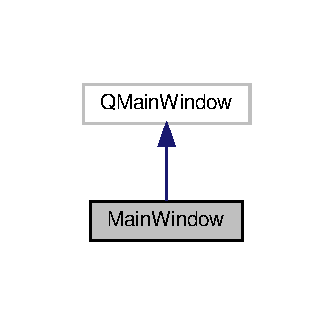
\includegraphics[width=160pt]{classMainWindow__inherit__graph}
\end{center}
\end{figure}


Collaboration diagram for Main\+Window\+:\nopagebreak
\begin{figure}[H]
\begin{center}
\leavevmode
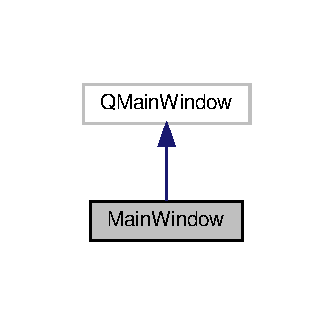
\includegraphics[width=160pt]{classMainWindow__coll__graph}
\end{center}
\end{figure}
\subsection*{Public Member Functions}
\begin{DoxyCompactItemize}
\item 
\mbox{\Hypertarget{classMainWindow_a996c5a2b6f77944776856f08ec30858d}\label{classMainWindow_a996c5a2b6f77944776856f08ec30858d}} 
{\bfseries Main\+Window} (Q\+Widget $\ast$parent=nullptr)
\end{DoxyCompactItemize}


The documentation for this class was generated from the following files\+:\begin{DoxyCompactItemize}
\item 
src/mainwindow.\+h\item 
src/mainwindow.\+cpp\end{DoxyCompactItemize}

\hypertarget{classOrder}{}\section{Order Class Reference}
\label{classOrder}\index{Order@{Order}}


The \hyperlink{classOrder}{Order} class.  




{\ttfamily \#include $<$Player\+Event.\+h$>$}



Inheritance diagram for Order\+:
\nopagebreak
\begin{figure}[H]
\begin{center}
\leavevmode
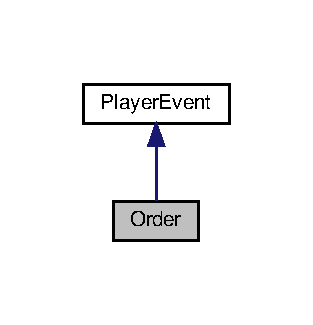
\includegraphics[width=150pt]{classOrder__inherit__graph}
\end{center}
\end{figure}


Collaboration diagram for Order\+:
\nopagebreak
\begin{figure}[H]
\begin{center}
\leavevmode
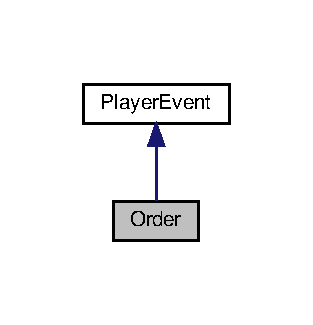
\includegraphics[width=150pt]{classOrder__coll__graph}
\end{center}
\end{figure}
\subsection*{Additional Inherited Members}


\subsection{Detailed Description}
The \hyperlink{classOrder}{Order} class. 

The documentation for this class was generated from the following file\+:\begin{DoxyCompactItemize}
\item 
src/Player\+Event.\+h\end{DoxyCompactItemize}

\hypertarget{classPlayer}{}\section{Player Class Reference}
\label{classPlayer}\index{Player@{Player}}


The \hyperlink{classPlayer}{Player} class.  




{\ttfamily \#include $<$player.\+h$>$}

\subsection*{Public Member Functions}
\begin{DoxyCompactItemize}
\item 
\hyperlink{classOrder}{Order} \hyperlink{classPlayer_a698698a4fc4ae46e2ee5085e1b132ee0}{place\+Order} (int number\+Of\+Beers)
\begin{DoxyCompactList}\small\item\em Method for placing order of beers. \end{DoxyCompactList}\item 
\hyperlink{classShipment}{Shipment} \hyperlink{classPlayer_abab9379aa93644769bbd93767f9eebdc}{place\+Shipment} (int number\+Of\+Beers)
\begin{DoxyCompactList}\small\item\em Method for shipment of beers placed. \end{DoxyCompactList}\item 
int \hyperlink{classPlayer_ae2197d1061a24fa444129b5ea85996d5}{decrease\+Inventory} (int number\+Of\+Beers)
\begin{DoxyCompactList}\small\item\em Method for decreasing inventory. \end{DoxyCompactList}\item 
int \hyperlink{classPlayer_af67e6ee0de38f3e9635d35849f103449}{increase\+Inventory} (int number\+Of\+Beers)
\begin{DoxyCompactList}\small\item\em Method for Increasing Inventory. \end{DoxyCompactList}\item 
void \hyperlink{classPlayer_ae1a59b99f054470c0e2fde589a29a559}{receive\+Shipment} (int number\+Of\+Beers)
\begin{DoxyCompactList}\small\item\em Method for Receiving shipment. \end{DoxyCompactList}\item 
void \hyperlink{classPlayer_af0df6a78d154f85b72869044a91adcf3}{receive\+Order} (int number\+Of\+Beers)
\begin{DoxyCompactList}\small\item\em Method for Reseiving order. \end{DoxyCompactList}\item 
int \hyperlink{classPlayer_a5e1a112bbb49e2896aa71aa8ffa02e90}{get\+Available\+Shipment} (unsigned int demand)
\begin{DoxyCompactList}\small\item\em Getter Method for Amount avalible shipment of beers. \end{DoxyCompactList}\item 
unsigned int \hyperlink{classPlayer_aec4626d021f2729c52306e7d303ddcff}{get\+P\+Id} () const
\begin{DoxyCompactList}\small\item\em Implementation of getters and setter for this class. \end{DoxyCompactList}\item 
void \hyperlink{classPlayer_a016beea94a91d74bc04d29088228316b}{set\+P\+Id} (unsigned int value)
\begin{DoxyCompactList}\small\item\em Setter Method for The player id. \end{DoxyCompactList}\item 
unsigned int \hyperlink{classPlayer_af78ce362224fb94149c6cf84dd34f9ea}{get\+Role} () const
\begin{DoxyCompactList}\small\item\em Getter Method for The player role. \end{DoxyCompactList}\item 
void \hyperlink{classPlayer_a008b3feee7ca705d7637cc3fbe5d7c58}{set\+Role} (unsigned int value)
\begin{DoxyCompactList}\small\item\em Setter Method for The player role. \end{DoxyCompactList}\item 
unsigned int \hyperlink{classPlayer_ade2a771c2e4a42560dae2acf2041ba8b}{get\+Demand} () const
\begin{DoxyCompactList}\small\item\em Getter Method for Amount of beers in demand. \end{DoxyCompactList}\item 
void \hyperlink{classPlayer_ad8d2808aaf6a627451a1d82f26d45812}{set\+Demand} (unsigned int value)
\begin{DoxyCompactList}\small\item\em Setter Method for Amount of beers in demand. \end{DoxyCompactList}\item 
bool \hyperlink{classPlayer_a266523063d6642e14894dec606f31e45}{get\+Order\+Placed} () const
\begin{DoxyCompactList}\small\item\em Getter Method to check if orderd placed or not. \end{DoxyCompactList}\item 
void \hyperlink{classPlayer_a1afe9b0b034e8c8544fc745abcf47448}{set\+Order\+Placed} (bool value)
\begin{DoxyCompactList}\small\item\em Setter Method for Amount of beers ordered. \end{DoxyCompactList}\item 
unsigned int \hyperlink{classPlayer_ac0da2a656e267a7f06be30c9e99d26e6}{get\+Inventory} () const
\begin{DoxyCompactList}\small\item\em Getter Method for Amount of beers in inventory. \end{DoxyCompactList}\item 
void \hyperlink{classPlayer_a26403ca486d7a34a5a27397eee42d531}{set\+Inventory} (unsigned int value)
\begin{DoxyCompactList}\small\item\em Setter Method for Amount of beers in inventory. \end{DoxyCompactList}\item 
unsigned int \hyperlink{classPlayer_a538ba7ec623afd550c37783c10957c3d}{get\+Backorder} () const
\begin{DoxyCompactList}\small\item\em Getter Method for Amount of beers in back order. \end{DoxyCompactList}\item 
void \hyperlink{classPlayer_a131897406c5504012015860b5de606f0}{set\+Backorder} (unsigned int value)
\begin{DoxyCompactList}\small\item\em Setter Method for Amount of beers in back order. \end{DoxyCompactList}\item 
double \hyperlink{classPlayer_a38cf576aa5a4020ed2fafe1aa9046fdd}{get\+Cost} () const
\begin{DoxyCompactList}\small\item\em Getter Method for Beer cost. \end{DoxyCompactList}\item 
void \hyperlink{classPlayer_a2fd1430d641ef17c52b0aae31e7e26bf}{set\+Cost} (double value)
\begin{DoxyCompactList}\small\item\em Setter Method for Beer cost. \end{DoxyCompactList}\item 
double \hyperlink{classPlayer_a0c5cd74a628ad6fb79ebb790dd1a956b}{get\+Total\+Cost} () const
\begin{DoxyCompactList}\small\item\em Getter Method for Total Beer cost. \end{DoxyCompactList}\item 
void \hyperlink{classPlayer_ab79475527bb480b01d004106580158b5}{set\+Total\+Cost} (double value)
\begin{DoxyCompactList}\small\item\em Setter Method for Total Beer cost. \end{DoxyCompactList}\item 
unsigned int \hyperlink{classPlayer_afd54f2f323e1430efda2acd30163e7ff}{get\+Outgoing\+Shipment} () const
\begin{DoxyCompactList}\small\item\em Getter Method for Amount of beers in outgoing shipment. \end{DoxyCompactList}\item 
void \hyperlink{classPlayer_aeed18c6e38773f2c8035b8604b38df29}{set\+Outgoing\+Shipment} (unsigned int value)
\begin{DoxyCompactList}\small\item\em Setter Method for Amount of beers in outgoingshipment. \end{DoxyCompactList}\item 
bool \hyperlink{classPlayer_a5be8afcdfb75792e300d9c255d058a05}{is\+Order\+Received} () const
\begin{DoxyCompactList}\small\item\em Getter Method to check if order received or not. \end{DoxyCompactList}\item 
void \hyperlink{classPlayer_abb73217aac5315b6d78c58feb25a88df}{set\+Order\+Received} (bool value)
\begin{DoxyCompactList}\small\item\em Setter Method to set order received to True or False. \end{DoxyCompactList}\item 
bool \hyperlink{classPlayer_ad3834057ec43f27a631d24f276586265}{is\+Shipment\+Received} () const
\begin{DoxyCompactList}\small\item\em Getter Method to check if shipment received or not. \end{DoxyCompactList}\item 
void \hyperlink{classPlayer_a6b24d6f3b7d11df39c621a2dfb4d19e4}{set\+Shipment\+Received} (bool value)
\begin{DoxyCompactList}\small\item\em Setter Method for Amount of shipment of beers received. \end{DoxyCompactList}\item 
bool \hyperlink{classPlayer_a90c450a83447d63a40c22eca44624121}{get\+Shipment\+Placed} () const
\begin{DoxyCompactList}\small\item\em Getter Method to check if shipment placed or not. \end{DoxyCompactList}\item 
void \hyperlink{classPlayer_ae6ff3d0d308302f5fc64071991e3cdda}{set\+Shipment\+Placed} (bool value)
\begin{DoxyCompactList}\small\item\em Setter Method to set shipment places to True or False. \end{DoxyCompactList}\end{DoxyCompactItemize}


\subsection{Detailed Description}
The \hyperlink{classPlayer}{Player} class. 

\subsection{Member Function Documentation}
\mbox{\Hypertarget{classPlayer_ae2197d1061a24fa444129b5ea85996d5}\label{classPlayer_ae2197d1061a24fa444129b5ea85996d5}} 
\index{Player@{Player}!decrease\+Inventory@{decrease\+Inventory}}
\index{decrease\+Inventory@{decrease\+Inventory}!Player@{Player}}
\subsubsection{\texorpdfstring{decrease\+Inventory()}{decreaseInventory()}}
{\footnotesize\ttfamily int Player\+::decrease\+Inventory (\begin{DoxyParamCaption}\item[{int}]{number\+Of\+Beers }\end{DoxyParamCaption})}



Method for decreasing inventory. 


\begin{DoxyParams}{Parameters}
{\em Amount} & of beers removed from inventory \\
\hline
\end{DoxyParams}
\begin{DoxyReturn}{Returns}
Amount of beers in inventory 
\end{DoxyReturn}
\mbox{\Hypertarget{classPlayer_a5e1a112bbb49e2896aa71aa8ffa02e90}\label{classPlayer_a5e1a112bbb49e2896aa71aa8ffa02e90}} 
\index{Player@{Player}!get\+Available\+Shipment@{get\+Available\+Shipment}}
\index{get\+Available\+Shipment@{get\+Available\+Shipment}!Player@{Player}}
\subsubsection{\texorpdfstring{get\+Available\+Shipment()}{getAvailableShipment()}}
{\footnotesize\ttfamily int Player\+::get\+Available\+Shipment (\begin{DoxyParamCaption}\item[{unsigned int}]{demand }\end{DoxyParamCaption})}



Getter Method for Amount avalible shipment of beers. 


\begin{DoxyParams}{Parameters}
{\em Amount} & of beers demanded for shipment \\
\hline
\end{DoxyParams}
\begin{DoxyReturn}{Returns}
Amount of beers avalible for shipment 
\end{DoxyReturn}
\mbox{\Hypertarget{classPlayer_a538ba7ec623afd550c37783c10957c3d}\label{classPlayer_a538ba7ec623afd550c37783c10957c3d}} 
\index{Player@{Player}!get\+Backorder@{get\+Backorder}}
\index{get\+Backorder@{get\+Backorder}!Player@{Player}}
\subsubsection{\texorpdfstring{get\+Backorder()}{getBackorder()}}
{\footnotesize\ttfamily unsigned int Player\+::get\+Backorder (\begin{DoxyParamCaption}{ }\end{DoxyParamCaption}) const}



Getter Method for Amount of beers in back order. 

\begin{DoxyReturn}{Returns}
Amount of beers in back order 
\end{DoxyReturn}
\mbox{\Hypertarget{classPlayer_a38cf576aa5a4020ed2fafe1aa9046fdd}\label{classPlayer_a38cf576aa5a4020ed2fafe1aa9046fdd}} 
\index{Player@{Player}!get\+Cost@{get\+Cost}}
\index{get\+Cost@{get\+Cost}!Player@{Player}}
\subsubsection{\texorpdfstring{get\+Cost()}{getCost()}}
{\footnotesize\ttfamily double Player\+::get\+Cost (\begin{DoxyParamCaption}{ }\end{DoxyParamCaption}) const}



Getter Method for Beer cost. 

\begin{DoxyReturn}{Returns}
Beer cost 
\end{DoxyReturn}
\mbox{\Hypertarget{classPlayer_ade2a771c2e4a42560dae2acf2041ba8b}\label{classPlayer_ade2a771c2e4a42560dae2acf2041ba8b}} 
\index{Player@{Player}!get\+Demand@{get\+Demand}}
\index{get\+Demand@{get\+Demand}!Player@{Player}}
\subsubsection{\texorpdfstring{get\+Demand()}{getDemand()}}
{\footnotesize\ttfamily unsigned int Player\+::get\+Demand (\begin{DoxyParamCaption}{ }\end{DoxyParamCaption}) const}



Getter Method for Amount of beers in demand. 

\begin{DoxyReturn}{Returns}
Amount of beers in demand 
\end{DoxyReturn}
\mbox{\Hypertarget{classPlayer_ac0da2a656e267a7f06be30c9e99d26e6}\label{classPlayer_ac0da2a656e267a7f06be30c9e99d26e6}} 
\index{Player@{Player}!get\+Inventory@{get\+Inventory}}
\index{get\+Inventory@{get\+Inventory}!Player@{Player}}
\subsubsection{\texorpdfstring{get\+Inventory()}{getInventory()}}
{\footnotesize\ttfamily unsigned int Player\+::get\+Inventory (\begin{DoxyParamCaption}{ }\end{DoxyParamCaption}) const}



Getter Method for Amount of beers in inventory. 

\begin{DoxyReturn}{Returns}
Amount of beers in inventory 
\end{DoxyReturn}
\mbox{\Hypertarget{classPlayer_a266523063d6642e14894dec606f31e45}\label{classPlayer_a266523063d6642e14894dec606f31e45}} 
\index{Player@{Player}!get\+Order\+Placed@{get\+Order\+Placed}}
\index{get\+Order\+Placed@{get\+Order\+Placed}!Player@{Player}}
\subsubsection{\texorpdfstring{get\+Order\+Placed()}{getOrderPlaced()}}
{\footnotesize\ttfamily bool Player\+::get\+Order\+Placed (\begin{DoxyParamCaption}{ }\end{DoxyParamCaption}) const}



Getter Method to check if orderd placed or not. 

\begin{DoxyReturn}{Returns}
True or False 
\end{DoxyReturn}
\mbox{\Hypertarget{classPlayer_afd54f2f323e1430efda2acd30163e7ff}\label{classPlayer_afd54f2f323e1430efda2acd30163e7ff}} 
\index{Player@{Player}!get\+Outgoing\+Shipment@{get\+Outgoing\+Shipment}}
\index{get\+Outgoing\+Shipment@{get\+Outgoing\+Shipment}!Player@{Player}}
\subsubsection{\texorpdfstring{get\+Outgoing\+Shipment()}{getOutgoingShipment()}}
{\footnotesize\ttfamily unsigned int Player\+::get\+Outgoing\+Shipment (\begin{DoxyParamCaption}{ }\end{DoxyParamCaption}) const}



Getter Method for Amount of beers in outgoing shipment. 

\begin{DoxyReturn}{Returns}
Amount of beers in outgoing shipment 
\end{DoxyReturn}
\mbox{\Hypertarget{classPlayer_aec4626d021f2729c52306e7d303ddcff}\label{classPlayer_aec4626d021f2729c52306e7d303ddcff}} 
\index{Player@{Player}!get\+P\+Id@{get\+P\+Id}}
\index{get\+P\+Id@{get\+P\+Id}!Player@{Player}}
\subsubsection{\texorpdfstring{get\+P\+Id()}{getPId()}}
{\footnotesize\ttfamily unsigned int Player\+::get\+P\+Id (\begin{DoxyParamCaption}{ }\end{DoxyParamCaption}) const}



Implementation of getters and setter for this class. 

Getter Method for The player id \begin{DoxyReturn}{Returns}
The player id 
\end{DoxyReturn}
\mbox{\Hypertarget{classPlayer_af78ce362224fb94149c6cf84dd34f9ea}\label{classPlayer_af78ce362224fb94149c6cf84dd34f9ea}} 
\index{Player@{Player}!get\+Role@{get\+Role}}
\index{get\+Role@{get\+Role}!Player@{Player}}
\subsubsection{\texorpdfstring{get\+Role()}{getRole()}}
{\footnotesize\ttfamily unsigned int Player\+::get\+Role (\begin{DoxyParamCaption}{ }\end{DoxyParamCaption}) const}



Getter Method for The player role. 

\begin{DoxyReturn}{Returns}
The player role 
\end{DoxyReturn}
\mbox{\Hypertarget{classPlayer_a90c450a83447d63a40c22eca44624121}\label{classPlayer_a90c450a83447d63a40c22eca44624121}} 
\index{Player@{Player}!get\+Shipment\+Placed@{get\+Shipment\+Placed}}
\index{get\+Shipment\+Placed@{get\+Shipment\+Placed}!Player@{Player}}
\subsubsection{\texorpdfstring{get\+Shipment\+Placed()}{getShipmentPlaced()}}
{\footnotesize\ttfamily bool Player\+::get\+Shipment\+Placed (\begin{DoxyParamCaption}{ }\end{DoxyParamCaption}) const}



Getter Method to check if shipment placed or not. 

\begin{DoxyReturn}{Returns}
True or False 
\end{DoxyReturn}
\mbox{\Hypertarget{classPlayer_a0c5cd74a628ad6fb79ebb790dd1a956b}\label{classPlayer_a0c5cd74a628ad6fb79ebb790dd1a956b}} 
\index{Player@{Player}!get\+Total\+Cost@{get\+Total\+Cost}}
\index{get\+Total\+Cost@{get\+Total\+Cost}!Player@{Player}}
\subsubsection{\texorpdfstring{get\+Total\+Cost()}{getTotalCost()}}
{\footnotesize\ttfamily double Player\+::get\+Total\+Cost (\begin{DoxyParamCaption}{ }\end{DoxyParamCaption}) const}



Getter Method for Total Beer cost. 

\begin{DoxyReturn}{Returns}
Total Beer cost 
\end{DoxyReturn}
\mbox{\Hypertarget{classPlayer_af67e6ee0de38f3e9635d35849f103449}\label{classPlayer_af67e6ee0de38f3e9635d35849f103449}} 
\index{Player@{Player}!increase\+Inventory@{increase\+Inventory}}
\index{increase\+Inventory@{increase\+Inventory}!Player@{Player}}
\subsubsection{\texorpdfstring{increase\+Inventory()}{increaseInventory()}}
{\footnotesize\ttfamily int Player\+::increase\+Inventory (\begin{DoxyParamCaption}\item[{int}]{number\+Of\+Beers }\end{DoxyParamCaption})}



Method for Increasing Inventory. 


\begin{DoxyParams}{Parameters}
{\em Amount} & of beers added to inventory \\
\hline
\end{DoxyParams}
\begin{DoxyReturn}{Returns}
Amount of beers in inventory 
\end{DoxyReturn}
\mbox{\Hypertarget{classPlayer_a5be8afcdfb75792e300d9c255d058a05}\label{classPlayer_a5be8afcdfb75792e300d9c255d058a05}} 
\index{Player@{Player}!is\+Order\+Received@{is\+Order\+Received}}
\index{is\+Order\+Received@{is\+Order\+Received}!Player@{Player}}
\subsubsection{\texorpdfstring{is\+Order\+Received()}{isOrderReceived()}}
{\footnotesize\ttfamily bool Player\+::is\+Order\+Received (\begin{DoxyParamCaption}{ }\end{DoxyParamCaption}) const}



Getter Method to check if order received or not. 

\begin{DoxyReturn}{Returns}
True or False 
\end{DoxyReturn}
\mbox{\Hypertarget{classPlayer_ad3834057ec43f27a631d24f276586265}\label{classPlayer_ad3834057ec43f27a631d24f276586265}} 
\index{Player@{Player}!is\+Shipment\+Received@{is\+Shipment\+Received}}
\index{is\+Shipment\+Received@{is\+Shipment\+Received}!Player@{Player}}
\subsubsection{\texorpdfstring{is\+Shipment\+Received()}{isShipmentReceived()}}
{\footnotesize\ttfamily bool Player\+::is\+Shipment\+Received (\begin{DoxyParamCaption}{ }\end{DoxyParamCaption}) const}



Getter Method to check if shipment received or not. 

\begin{DoxyReturn}{Returns}
Trur or False 
\end{DoxyReturn}
\mbox{\Hypertarget{classPlayer_a698698a4fc4ae46e2ee5085e1b132ee0}\label{classPlayer_a698698a4fc4ae46e2ee5085e1b132ee0}} 
\index{Player@{Player}!place\+Order@{place\+Order}}
\index{place\+Order@{place\+Order}!Player@{Player}}
\subsubsection{\texorpdfstring{place\+Order()}{placeOrder()}}
{\footnotesize\ttfamily \hyperlink{classOrder}{Order} Player\+::place\+Order (\begin{DoxyParamCaption}\item[{int}]{number\+Of\+Beers }\end{DoxyParamCaption})}



Method for placing order of beers. 


\begin{DoxyParams}{Parameters}
{\em Amount} & of beers orderd \\
\hline
\end{DoxyParams}
\begin{DoxyReturn}{Returns}
\hyperlink{classOrder}{Order} 
\end{DoxyReturn}
\mbox{\Hypertarget{classPlayer_abab9379aa93644769bbd93767f9eebdc}\label{classPlayer_abab9379aa93644769bbd93767f9eebdc}} 
\index{Player@{Player}!place\+Shipment@{place\+Shipment}}
\index{place\+Shipment@{place\+Shipment}!Player@{Player}}
\subsubsection{\texorpdfstring{place\+Shipment()}{placeShipment()}}
{\footnotesize\ttfamily \hyperlink{classShipment}{Shipment} Player\+::place\+Shipment (\begin{DoxyParamCaption}\item[{int}]{number\+Of\+Beers }\end{DoxyParamCaption})}



Method for shipment of beers placed. 


\begin{DoxyParams}{Parameters}
{\em Amount} & of beers avaliblr for shipment \\
\hline
\end{DoxyParams}
\begin{DoxyReturn}{Returns}
void 
\end{DoxyReturn}
\mbox{\Hypertarget{classPlayer_af0df6a78d154f85b72869044a91adcf3}\label{classPlayer_af0df6a78d154f85b72869044a91adcf3}} 
\index{Player@{Player}!receive\+Order@{receive\+Order}}
\index{receive\+Order@{receive\+Order}!Player@{Player}}
\subsubsection{\texorpdfstring{receive\+Order()}{receiveOrder()}}
{\footnotesize\ttfamily void Player\+::receive\+Order (\begin{DoxyParamCaption}\item[{int}]{number\+Of\+Beers }\end{DoxyParamCaption})}



Method for Reseiving order. 


\begin{DoxyParams}{Parameters}
{\em Amount} & of beers received \\
\hline
\end{DoxyParams}
\begin{DoxyReturn}{Returns}
void 
\end{DoxyReturn}
\mbox{\Hypertarget{classPlayer_ae1a59b99f054470c0e2fde589a29a559}\label{classPlayer_ae1a59b99f054470c0e2fde589a29a559}} 
\index{Player@{Player}!receive\+Shipment@{receive\+Shipment}}
\index{receive\+Shipment@{receive\+Shipment}!Player@{Player}}
\subsubsection{\texorpdfstring{receive\+Shipment()}{receiveShipment()}}
{\footnotesize\ttfamily void Player\+::receive\+Shipment (\begin{DoxyParamCaption}\item[{int}]{number\+Of\+Beers }\end{DoxyParamCaption})}



Method for Receiving shipment. 


\begin{DoxyParams}{Parameters}
{\em Amount} & of beers received by shipment \\
\hline
\end{DoxyParams}
\begin{DoxyReturn}{Returns}
void 
\end{DoxyReturn}
\mbox{\Hypertarget{classPlayer_a131897406c5504012015860b5de606f0}\label{classPlayer_a131897406c5504012015860b5de606f0}} 
\index{Player@{Player}!set\+Backorder@{set\+Backorder}}
\index{set\+Backorder@{set\+Backorder}!Player@{Player}}
\subsubsection{\texorpdfstring{set\+Backorder()}{setBackorder()}}
{\footnotesize\ttfamily void Player\+::set\+Backorder (\begin{DoxyParamCaption}\item[{unsigned int}]{value }\end{DoxyParamCaption})}



Setter Method for Amount of beers in back order. 


\begin{DoxyParams}{Parameters}
{\em value} & Amount of beers in back order \\
\hline
\end{DoxyParams}
\begin{DoxyReturn}{Returns}
void 
\end{DoxyReturn}
\mbox{\Hypertarget{classPlayer_a2fd1430d641ef17c52b0aae31e7e26bf}\label{classPlayer_a2fd1430d641ef17c52b0aae31e7e26bf}} 
\index{Player@{Player}!set\+Cost@{set\+Cost}}
\index{set\+Cost@{set\+Cost}!Player@{Player}}
\subsubsection{\texorpdfstring{set\+Cost()}{setCost()}}
{\footnotesize\ttfamily void Player\+::set\+Cost (\begin{DoxyParamCaption}\item[{double}]{value }\end{DoxyParamCaption})}



Setter Method for Beer cost. 


\begin{DoxyParams}{Parameters}
{\em value} & Beer cost \\
\hline
\end{DoxyParams}
\begin{DoxyReturn}{Returns}
void 
\end{DoxyReturn}
\mbox{\Hypertarget{classPlayer_ad8d2808aaf6a627451a1d82f26d45812}\label{classPlayer_ad8d2808aaf6a627451a1d82f26d45812}} 
\index{Player@{Player}!set\+Demand@{set\+Demand}}
\index{set\+Demand@{set\+Demand}!Player@{Player}}
\subsubsection{\texorpdfstring{set\+Demand()}{setDemand()}}
{\footnotesize\ttfamily void Player\+::set\+Demand (\begin{DoxyParamCaption}\item[{unsigned int}]{value }\end{DoxyParamCaption})}



Setter Method for Amount of beers in demand. 


\begin{DoxyParams}{Parameters}
{\em value} & Amount of beers in demand \\
\hline
\end{DoxyParams}
\begin{DoxyReturn}{Returns}
void 
\end{DoxyReturn}
\mbox{\Hypertarget{classPlayer_a26403ca486d7a34a5a27397eee42d531}\label{classPlayer_a26403ca486d7a34a5a27397eee42d531}} 
\index{Player@{Player}!set\+Inventory@{set\+Inventory}}
\index{set\+Inventory@{set\+Inventory}!Player@{Player}}
\subsubsection{\texorpdfstring{set\+Inventory()}{setInventory()}}
{\footnotesize\ttfamily void Player\+::set\+Inventory (\begin{DoxyParamCaption}\item[{unsigned int}]{value }\end{DoxyParamCaption})}



Setter Method for Amount of beers in inventory. 


\begin{DoxyParams}{Parameters}
{\em value} & Amount of beers in inventory \\
\hline
\end{DoxyParams}
\begin{DoxyReturn}{Returns}
void 
\end{DoxyReturn}
\mbox{\Hypertarget{classPlayer_a1afe9b0b034e8c8544fc745abcf47448}\label{classPlayer_a1afe9b0b034e8c8544fc745abcf47448}} 
\index{Player@{Player}!set\+Order\+Placed@{set\+Order\+Placed}}
\index{set\+Order\+Placed@{set\+Order\+Placed}!Player@{Player}}
\subsubsection{\texorpdfstring{set\+Order\+Placed()}{setOrderPlaced()}}
{\footnotesize\ttfamily void Player\+::set\+Order\+Placed (\begin{DoxyParamCaption}\item[{bool}]{value }\end{DoxyParamCaption})}



Setter Method for Amount of beers ordered. 


\begin{DoxyParams}{Parameters}
{\em value} & Amount of beers ordered \\
\hline
\end{DoxyParams}
\begin{DoxyReturn}{Returns}
void 
\end{DoxyReturn}
\mbox{\Hypertarget{classPlayer_abb73217aac5315b6d78c58feb25a88df}\label{classPlayer_abb73217aac5315b6d78c58feb25a88df}} 
\index{Player@{Player}!set\+Order\+Received@{set\+Order\+Received}}
\index{set\+Order\+Received@{set\+Order\+Received}!Player@{Player}}
\subsubsection{\texorpdfstring{set\+Order\+Received()}{setOrderReceived()}}
{\footnotesize\ttfamily void Player\+::set\+Order\+Received (\begin{DoxyParamCaption}\item[{bool}]{value }\end{DoxyParamCaption})}



Setter Method to set order received to True or False. 


\begin{DoxyParams}{Parameters}
{\em True} & or False \\
\hline
\end{DoxyParams}
\begin{DoxyReturn}{Returns}
void 
\end{DoxyReturn}
\mbox{\Hypertarget{classPlayer_aeed18c6e38773f2c8035b8604b38df29}\label{classPlayer_aeed18c6e38773f2c8035b8604b38df29}} 
\index{Player@{Player}!set\+Outgoing\+Shipment@{set\+Outgoing\+Shipment}}
\index{set\+Outgoing\+Shipment@{set\+Outgoing\+Shipment}!Player@{Player}}
\subsubsection{\texorpdfstring{set\+Outgoing\+Shipment()}{setOutgoingShipment()}}
{\footnotesize\ttfamily void Player\+::set\+Outgoing\+Shipment (\begin{DoxyParamCaption}\item[{unsigned int}]{value }\end{DoxyParamCaption})}



Setter Method for Amount of beers in outgoingshipment. 


\begin{DoxyParams}{Parameters}
{\em value} & Amount of beers in outgoing shipment \\
\hline
\end{DoxyParams}
\begin{DoxyReturn}{Returns}
void 
\end{DoxyReturn}
\mbox{\Hypertarget{classPlayer_a016beea94a91d74bc04d29088228316b}\label{classPlayer_a016beea94a91d74bc04d29088228316b}} 
\index{Player@{Player}!set\+P\+Id@{set\+P\+Id}}
\index{set\+P\+Id@{set\+P\+Id}!Player@{Player}}
\subsubsection{\texorpdfstring{set\+P\+Id()}{setPId()}}
{\footnotesize\ttfamily void Player\+::set\+P\+Id (\begin{DoxyParamCaption}\item[{unsigned int}]{value }\end{DoxyParamCaption})}



Setter Method for The player id. 


\begin{DoxyParams}{Parameters}
{\em value} & The player id \\
\hline
\end{DoxyParams}
\begin{DoxyReturn}{Returns}
void 
\end{DoxyReturn}
\mbox{\Hypertarget{classPlayer_a008b3feee7ca705d7637cc3fbe5d7c58}\label{classPlayer_a008b3feee7ca705d7637cc3fbe5d7c58}} 
\index{Player@{Player}!set\+Role@{set\+Role}}
\index{set\+Role@{set\+Role}!Player@{Player}}
\subsubsection{\texorpdfstring{set\+Role()}{setRole()}}
{\footnotesize\ttfamily void Player\+::set\+Role (\begin{DoxyParamCaption}\item[{unsigned int}]{value }\end{DoxyParamCaption})}



Setter Method for The player role. 


\begin{DoxyParams}{Parameters}
{\em value} & The player role \\
\hline
\end{DoxyParams}
\begin{DoxyReturn}{Returns}
void 
\end{DoxyReturn}
\mbox{\Hypertarget{classPlayer_ae6ff3d0d308302f5fc64071991e3cdda}\label{classPlayer_ae6ff3d0d308302f5fc64071991e3cdda}} 
\index{Player@{Player}!set\+Shipment\+Placed@{set\+Shipment\+Placed}}
\index{set\+Shipment\+Placed@{set\+Shipment\+Placed}!Player@{Player}}
\subsubsection{\texorpdfstring{set\+Shipment\+Placed()}{setShipmentPlaced()}}
{\footnotesize\ttfamily void Player\+::set\+Shipment\+Placed (\begin{DoxyParamCaption}\item[{bool}]{value }\end{DoxyParamCaption})}



Setter Method to set shipment places to True or False. 


\begin{DoxyParams}{Parameters}
{\em True} & or False \\
\hline
\end{DoxyParams}
\begin{DoxyReturn}{Returns}
void 
\end{DoxyReturn}
\mbox{\Hypertarget{classPlayer_a6b24d6f3b7d11df39c621a2dfb4d19e4}\label{classPlayer_a6b24d6f3b7d11df39c621a2dfb4d19e4}} 
\index{Player@{Player}!set\+Shipment\+Received@{set\+Shipment\+Received}}
\index{set\+Shipment\+Received@{set\+Shipment\+Received}!Player@{Player}}
\subsubsection{\texorpdfstring{set\+Shipment\+Received()}{setShipmentReceived()}}
{\footnotesize\ttfamily void Player\+::set\+Shipment\+Received (\begin{DoxyParamCaption}\item[{bool}]{value }\end{DoxyParamCaption})}



Setter Method for Amount of shipment of beers received. 


\begin{DoxyParams}{Parameters}
{\em True} & or False \\
\hline
\end{DoxyParams}
\begin{DoxyReturn}{Returns}
void 
\end{DoxyReturn}
\mbox{\Hypertarget{classPlayer_ab79475527bb480b01d004106580158b5}\label{classPlayer_ab79475527bb480b01d004106580158b5}} 
\index{Player@{Player}!set\+Total\+Cost@{set\+Total\+Cost}}
\index{set\+Total\+Cost@{set\+Total\+Cost}!Player@{Player}}
\subsubsection{\texorpdfstring{set\+Total\+Cost()}{setTotalCost()}}
{\footnotesize\ttfamily void Player\+::set\+Total\+Cost (\begin{DoxyParamCaption}\item[{double}]{value }\end{DoxyParamCaption})}



Setter Method for Total Beer cost. 


\begin{DoxyParams}{Parameters}
{\em value} & Total Beer cost \\
\hline
\end{DoxyParams}
\begin{DoxyReturn}{Returns}
void 
\end{DoxyReturn}


The documentation for this class was generated from the following files\+:\begin{DoxyCompactItemize}
\item 
src/\hyperlink{player_8h}{player.\+h}\item 
src/player.\+cpp\end{DoxyCompactItemize}

\hypertarget{classplayerDialog}{}\section{player\+Dialog Class Reference}
\label{classplayerDialog}\index{player\+Dialog@{player\+Dialog}}


Inheritance diagram for player\+Dialog\+:\nopagebreak
\begin{figure}[H]
\begin{center}
\leavevmode
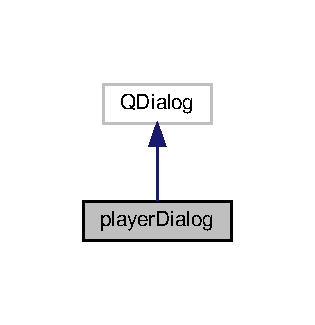
\includegraphics[width=151pt]{classplayerDialog__inherit__graph}
\end{center}
\end{figure}


Collaboration diagram for player\+Dialog\+:\nopagebreak
\begin{figure}[H]
\begin{center}
\leavevmode
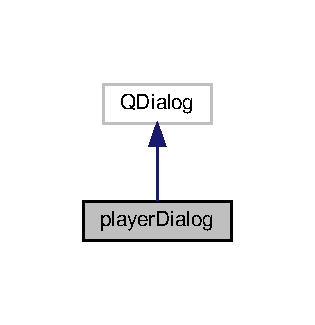
\includegraphics[width=151pt]{classplayerDialog__coll__graph}
\end{center}
\end{figure}
\subsection*{Public Member Functions}
\begin{DoxyCompactItemize}
\item 
\mbox{\Hypertarget{classplayerDialog_af0b84f32ec1181d738247502470e4d5e}\label{classplayerDialog_af0b84f32ec1181d738247502470e4d5e}} 
{\bfseries player\+Dialog} (Q\+Widget $\ast$parent=nullptr)
\end{DoxyCompactItemize}


The documentation for this class was generated from the following files\+:\begin{DoxyCompactItemize}
\item 
src/playerdialog.\+h\item 
src/playerdialog.\+cpp\end{DoxyCompactItemize}

\hypertarget{classPlayerEvent}{}\section{Player\+Event Class Reference}
\label{classPlayerEvent}\index{Player\+Event@{Player\+Event}}


The \hyperlink{classPlayerEvent}{Player\+Event} class.  




{\ttfamily \#include $<$Player\+Event.\+h$>$}



Inheritance diagram for Player\+Event\+:\nopagebreak
\begin{figure}[H]
\begin{center}
\leavevmode
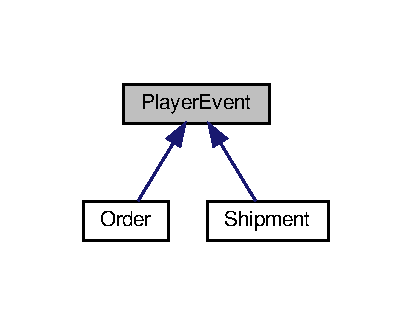
\includegraphics[width=198pt]{classPlayerEvent__inherit__graph}
\end{center}
\end{figure}
\subsection*{Public Member Functions}
\begin{DoxyCompactItemize}
\item 
unsigned int \hyperlink{classPlayerEvent_a9313159916c282a20bd69e27b6900679}{get\+Order\+Id} () const
\begin{DoxyCompactList}\small\item\em Implementation of getters and setter for this class. \end{DoxyCompactList}\item 
void \hyperlink{classPlayerEvent_ac1e16d56dfbd072f4bf5d2f73247ff38}{set\+Order\+Id} (unsigned int value)
\begin{DoxyCompactList}\small\item\em Setter Method for the order id. \end{DoxyCompactList}\item 
unsigned int \hyperlink{classPlayerEvent_ab44a2b22c16007d332524231089a9cc1}{get\+G\+Id} () const
\begin{DoxyCompactList}\small\item\em Getter Method for gid. \end{DoxyCompactList}\item 
void \hyperlink{classPlayerEvent_add2e994da90382443c45d533cbffa629}{set\+G\+Id} (unsigned int value)
\begin{DoxyCompactList}\small\item\em Setter Method for game id. \end{DoxyCompactList}\item 
unsigned int \hyperlink{classPlayerEvent_abc4c20973a6eafd4e9628c7264a1702d}{get\+From\+Player\+Id} () const
\begin{DoxyCompactList}\small\item\em Setter Method for game id. \end{DoxyCompactList}\item 
void \hyperlink{classPlayerEvent_a079ed27776a87240c7ac7700f1090df2}{set\+From\+Player\+Id} (unsigned int val)
\begin{DoxyCompactList}\small\item\em Setter Method for from\+Player\+Id. \end{DoxyCompactList}\item 
unsigned int \hyperlink{classPlayerEvent_a341da1afa86a54b8b5f242a7fc071fdc}{get\+To\+Player\+Id} () const
\begin{DoxyCompactList}\small\item\em Getter Method for player id for the beer to get shipped to. \end{DoxyCompactList}\item 
void \hyperlink{classPlayerEvent_ab867bb56d8a0cbf9c701a12f8c48987d}{set\+To\+Player\+Id} (unsigned int value)
\begin{DoxyCompactList}\small\item\em Setter Method for set\+To\+Player\+Id. \end{DoxyCompactList}\item 
unsigned int \hyperlink{classPlayerEvent_a9b9f5598c419cebae94fed31d209a09b}{get\+Ordered\+In\+Week} () const
\begin{DoxyCompactList}\small\item\em Getter Method for ordered in week. \end{DoxyCompactList}\item 
void \hyperlink{classPlayerEvent_ab6c0f61508410d40ff485de1c76095f1}{set\+Ordered\+In\+Week} (unsigned int value)
\begin{DoxyCompactList}\small\item\em Setter Method for the beers ordered in week. \end{DoxyCompactList}\item 
unsigned int \hyperlink{classPlayerEvent_ab541b87f6c0de2c990c2602b10d2b7cc}{get\+Shipped\+In\+Week} () const
\begin{DoxyCompactList}\small\item\em Getter Method for The beers shipped in week. \end{DoxyCompactList}\item 
void \hyperlink{classPlayerEvent_ac84be24b1509dfbedce45a78b33426d2}{set\+Shipped\+In\+Week} (unsigned int value)
\begin{DoxyCompactList}\small\item\em Setter Method for The beers shipped in week. \end{DoxyCompactList}\item 
unsigned int \hyperlink{classPlayerEvent_aebdec1d24172c7d3cefa6e76ac51f490}{get\+Number\+Of\+Beers} () const
\begin{DoxyCompactList}\small\item\em Getter Method for the numbers of beer. \end{DoxyCompactList}\item 
void \hyperlink{classPlayerEvent_a8c210ab3387262a7ecb17b16fe049593}{set\+Number\+Of\+Beers} (unsigned int value)
\begin{DoxyCompactList}\small\item\em Setter Method for the numbers of beer. \end{DoxyCompactList}\end{DoxyCompactItemize}
\subsection*{Protected Attributes}
\begin{DoxyCompactItemize}
\item 
\mbox{\Hypertarget{classPlayerEvent_abdd09cb025a56799d331736c94abcbad}\label{classPlayerEvent_abdd09cb025a56799d331736c94abcbad}} 
unsigned int \hyperlink{classPlayerEvent_abdd09cb025a56799d331736c94abcbad}{order\+Id}
\begin{DoxyCompactList}\small\item\em The order id. \end{DoxyCompactList}\item 
\mbox{\Hypertarget{classPlayerEvent_a16c8dca1a40b4922a320829808fb9d13}\label{classPlayerEvent_a16c8dca1a40b4922a320829808fb9d13}} 
unsigned int \hyperlink{classPlayerEvent_a16c8dca1a40b4922a320829808fb9d13}{gid}
\begin{DoxyCompactList}\small\item\em The gid. \end{DoxyCompactList}\item 
\mbox{\Hypertarget{classPlayerEvent_afdd7834bba00e55258afdfe0aa433efd}\label{classPlayerEvent_afdd7834bba00e55258afdfe0aa433efd}} 
unsigned int \hyperlink{classPlayerEvent_afdd7834bba00e55258afdfe0aa433efd}{from\+Playerid}
\begin{DoxyCompactList}\small\item\em The order from a player. \end{DoxyCompactList}\item 
\mbox{\Hypertarget{classPlayerEvent_a596b915ab8a814b4afde7cbe90737719}\label{classPlayerEvent_a596b915ab8a814b4afde7cbe90737719}} 
unsigned int \hyperlink{classPlayerEvent_a596b915ab8a814b4afde7cbe90737719}{to\+Playerid}
\begin{DoxyCompactList}\small\item\em The order to a player. \end{DoxyCompactList}\item 
\mbox{\Hypertarget{classPlayerEvent_ad5460958dd5953366aa7f72d3e09f6c1}\label{classPlayerEvent_ad5460958dd5953366aa7f72d3e09f6c1}} 
unsigned int \hyperlink{classPlayerEvent_ad5460958dd5953366aa7f72d3e09f6c1}{ordered\+In\+Week}
\begin{DoxyCompactList}\small\item\em The order in week. \end{DoxyCompactList}\item 
\mbox{\Hypertarget{classPlayerEvent_a893022c9784e236b67061cfe5e96ef45}\label{classPlayerEvent_a893022c9784e236b67061cfe5e96ef45}} 
unsigned int \hyperlink{classPlayerEvent_a893022c9784e236b67061cfe5e96ef45}{shipped\+In\+Week}
\begin{DoxyCompactList}\small\item\em The shipped in week. \end{DoxyCompactList}\item 
\mbox{\Hypertarget{classPlayerEvent_ad0148e813c51946a3c95efb3a09b1fe8}\label{classPlayerEvent_ad0148e813c51946a3c95efb3a09b1fe8}} 
unsigned int \hyperlink{classPlayerEvent_ad0148e813c51946a3c95efb3a09b1fe8}{number\+Of\+Beers}
\begin{DoxyCompactList}\small\item\em The order\textquotesingle{}s number of beers. \end{DoxyCompactList}\end{DoxyCompactItemize}


\subsection{Detailed Description}
The \hyperlink{classPlayerEvent}{Player\+Event} class. 

\subsection{Member Function Documentation}
\mbox{\Hypertarget{classPlayerEvent_abc4c20973a6eafd4e9628c7264a1702d}\label{classPlayerEvent_abc4c20973a6eafd4e9628c7264a1702d}} 
\index{Player\+Event@{Player\+Event}!get\+From\+Player\+Id@{get\+From\+Player\+Id}}
\index{get\+From\+Player\+Id@{get\+From\+Player\+Id}!Player\+Event@{Player\+Event}}
\subsubsection{\texorpdfstring{get\+From\+Player\+Id()}{getFromPlayerId()}}
{\footnotesize\ttfamily unsigned int Player\+Event\+::get\+From\+Player\+Id (\begin{DoxyParamCaption}{ }\end{DoxyParamCaption}) const}



Setter Method for game id. 


\begin{DoxyParams}{Parameters}
{\em value} & the game id of the order \\
\hline
\end{DoxyParams}
\begin{DoxyReturn}{Returns}
void 
\end{DoxyReturn}
\mbox{\Hypertarget{classPlayerEvent_ab44a2b22c16007d332524231089a9cc1}\label{classPlayerEvent_ab44a2b22c16007d332524231089a9cc1}} 
\index{Player\+Event@{Player\+Event}!get\+G\+Id@{get\+G\+Id}}
\index{get\+G\+Id@{get\+G\+Id}!Player\+Event@{Player\+Event}}
\subsubsection{\texorpdfstring{get\+G\+Id()}{getGId()}}
{\footnotesize\ttfamily unsigned int Player\+Event\+::get\+G\+Id (\begin{DoxyParamCaption}{ }\end{DoxyParamCaption}) const}



Getter Method for gid. 

\begin{DoxyReturn}{Returns}
gid 
\end{DoxyReturn}
\mbox{\Hypertarget{classPlayerEvent_aebdec1d24172c7d3cefa6e76ac51f490}\label{classPlayerEvent_aebdec1d24172c7d3cefa6e76ac51f490}} 
\index{Player\+Event@{Player\+Event}!get\+Number\+Of\+Beers@{get\+Number\+Of\+Beers}}
\index{get\+Number\+Of\+Beers@{get\+Number\+Of\+Beers}!Player\+Event@{Player\+Event}}
\subsubsection{\texorpdfstring{get\+Number\+Of\+Beers()}{getNumberOfBeers()}}
{\footnotesize\ttfamily unsigned int Player\+Event\+::get\+Number\+Of\+Beers (\begin{DoxyParamCaption}{ }\end{DoxyParamCaption}) const}



Getter Method for the numbers of beer. 

\begin{DoxyReturn}{Returns}
The numbers of beer 
\end{DoxyReturn}
\mbox{\Hypertarget{classPlayerEvent_a9b9f5598c419cebae94fed31d209a09b}\label{classPlayerEvent_a9b9f5598c419cebae94fed31d209a09b}} 
\index{Player\+Event@{Player\+Event}!get\+Ordered\+In\+Week@{get\+Ordered\+In\+Week}}
\index{get\+Ordered\+In\+Week@{get\+Ordered\+In\+Week}!Player\+Event@{Player\+Event}}
\subsubsection{\texorpdfstring{get\+Ordered\+In\+Week()}{getOrderedInWeek()}}
{\footnotesize\ttfamily unsigned int Player\+Event\+::get\+Ordered\+In\+Week (\begin{DoxyParamCaption}{ }\end{DoxyParamCaption}) const}



Getter Method for ordered in week. 

\begin{DoxyReturn}{Returns}
The beers ordered in week 
\end{DoxyReturn}
\mbox{\Hypertarget{classPlayerEvent_a9313159916c282a20bd69e27b6900679}\label{classPlayerEvent_a9313159916c282a20bd69e27b6900679}} 
\index{Player\+Event@{Player\+Event}!get\+Order\+Id@{get\+Order\+Id}}
\index{get\+Order\+Id@{get\+Order\+Id}!Player\+Event@{Player\+Event}}
\subsubsection{\texorpdfstring{get\+Order\+Id()}{getOrderId()}}
{\footnotesize\ttfamily unsigned int Player\+Event\+::get\+Order\+Id (\begin{DoxyParamCaption}{ }\end{DoxyParamCaption}) const}



Implementation of getters and setter for this class. 

Getter Method for the order id \begin{DoxyReturn}{Returns}
The order id 
\end{DoxyReturn}
\mbox{\Hypertarget{classPlayerEvent_ab541b87f6c0de2c990c2602b10d2b7cc}\label{classPlayerEvent_ab541b87f6c0de2c990c2602b10d2b7cc}} 
\index{Player\+Event@{Player\+Event}!get\+Shipped\+In\+Week@{get\+Shipped\+In\+Week}}
\index{get\+Shipped\+In\+Week@{get\+Shipped\+In\+Week}!Player\+Event@{Player\+Event}}
\subsubsection{\texorpdfstring{get\+Shipped\+In\+Week()}{getShippedInWeek()}}
{\footnotesize\ttfamily unsigned int Player\+Event\+::get\+Shipped\+In\+Week (\begin{DoxyParamCaption}{ }\end{DoxyParamCaption}) const}



Getter Method for The beers shipped in week. 

\begin{DoxyReturn}{Returns}
The beers shipped in week 
\end{DoxyReturn}
\mbox{\Hypertarget{classPlayerEvent_a341da1afa86a54b8b5f242a7fc071fdc}\label{classPlayerEvent_a341da1afa86a54b8b5f242a7fc071fdc}} 
\index{Player\+Event@{Player\+Event}!get\+To\+Player\+Id@{get\+To\+Player\+Id}}
\index{get\+To\+Player\+Id@{get\+To\+Player\+Id}!Player\+Event@{Player\+Event}}
\subsubsection{\texorpdfstring{get\+To\+Player\+Id()}{getToPlayerId()}}
{\footnotesize\ttfamily unsigned int Player\+Event\+::get\+To\+Player\+Id (\begin{DoxyParamCaption}{ }\end{DoxyParamCaption}) const}



Getter Method for player id for the beer to get shipped to. 

\begin{DoxyReturn}{Returns}
player id for the beer to get shipped to 
\end{DoxyReturn}
\mbox{\Hypertarget{classPlayerEvent_a079ed27776a87240c7ac7700f1090df2}\label{classPlayerEvent_a079ed27776a87240c7ac7700f1090df2}} 
\index{Player\+Event@{Player\+Event}!set\+From\+Player\+Id@{set\+From\+Player\+Id}}
\index{set\+From\+Player\+Id@{set\+From\+Player\+Id}!Player\+Event@{Player\+Event}}
\subsubsection{\texorpdfstring{set\+From\+Player\+Id()}{setFromPlayerId()}}
{\footnotesize\ttfamily void Player\+Event\+::set\+From\+Player\+Id (\begin{DoxyParamCaption}\item[{unsigned int}]{val }\end{DoxyParamCaption})}



Setter Method for from\+Player\+Id. 


\begin{DoxyParams}{Parameters}
{\em value} & the From \hyperlink{classPlayer}{Player} id \\
\hline
\end{DoxyParams}
\begin{DoxyReturn}{Returns}
void 
\end{DoxyReturn}
\mbox{\Hypertarget{classPlayerEvent_add2e994da90382443c45d533cbffa629}\label{classPlayerEvent_add2e994da90382443c45d533cbffa629}} 
\index{Player\+Event@{Player\+Event}!set\+G\+Id@{set\+G\+Id}}
\index{set\+G\+Id@{set\+G\+Id}!Player\+Event@{Player\+Event}}
\subsubsection{\texorpdfstring{set\+G\+Id()}{setGId()}}
{\footnotesize\ttfamily void Player\+Event\+::set\+G\+Id (\begin{DoxyParamCaption}\item[{unsigned int}]{value }\end{DoxyParamCaption})}



Setter Method for game id. 


\begin{DoxyParams}{Parameters}
{\em value} & the game id of the order \\
\hline
\end{DoxyParams}
\begin{DoxyReturn}{Returns}
void 
\end{DoxyReturn}
\mbox{\Hypertarget{classPlayerEvent_a8c210ab3387262a7ecb17b16fe049593}\label{classPlayerEvent_a8c210ab3387262a7ecb17b16fe049593}} 
\index{Player\+Event@{Player\+Event}!set\+Number\+Of\+Beers@{set\+Number\+Of\+Beers}}
\index{set\+Number\+Of\+Beers@{set\+Number\+Of\+Beers}!Player\+Event@{Player\+Event}}
\subsubsection{\texorpdfstring{set\+Number\+Of\+Beers()}{setNumberOfBeers()}}
{\footnotesize\ttfamily void Player\+Event\+::set\+Number\+Of\+Beers (\begin{DoxyParamCaption}\item[{unsigned int}]{value }\end{DoxyParamCaption})}



Setter Method for the numbers of beer. 


\begin{DoxyParams}{Parameters}
{\em value} & The numbers of beer \\
\hline
\end{DoxyParams}
\begin{DoxyReturn}{Returns}
void 
\end{DoxyReturn}
\mbox{\Hypertarget{classPlayerEvent_ab6c0f61508410d40ff485de1c76095f1}\label{classPlayerEvent_ab6c0f61508410d40ff485de1c76095f1}} 
\index{Player\+Event@{Player\+Event}!set\+Ordered\+In\+Week@{set\+Ordered\+In\+Week}}
\index{set\+Ordered\+In\+Week@{set\+Ordered\+In\+Week}!Player\+Event@{Player\+Event}}
\subsubsection{\texorpdfstring{set\+Ordered\+In\+Week()}{setOrderedInWeek()}}
{\footnotesize\ttfamily void Player\+Event\+::set\+Ordered\+In\+Week (\begin{DoxyParamCaption}\item[{unsigned int}]{value }\end{DoxyParamCaption})}



Setter Method for the beers ordered in week. 


\begin{DoxyParams}{Parameters}
{\em value} & The beers ordered in week \\
\hline
\end{DoxyParams}
\begin{DoxyReturn}{Returns}
void 
\end{DoxyReturn}
\mbox{\Hypertarget{classPlayerEvent_ac1e16d56dfbd072f4bf5d2f73247ff38}\label{classPlayerEvent_ac1e16d56dfbd072f4bf5d2f73247ff38}} 
\index{Player\+Event@{Player\+Event}!set\+Order\+Id@{set\+Order\+Id}}
\index{set\+Order\+Id@{set\+Order\+Id}!Player\+Event@{Player\+Event}}
\subsubsection{\texorpdfstring{set\+Order\+Id()}{setOrderId()}}
{\footnotesize\ttfamily void Player\+Event\+::set\+Order\+Id (\begin{DoxyParamCaption}\item[{unsigned int}]{value }\end{DoxyParamCaption})}



Setter Method for the order id. 


\begin{DoxyParams}{Parameters}
{\em value} & The order id \\
\hline
\end{DoxyParams}
\begin{DoxyReturn}{Returns}
void 
\end{DoxyReturn}
\mbox{\Hypertarget{classPlayerEvent_ac84be24b1509dfbedce45a78b33426d2}\label{classPlayerEvent_ac84be24b1509dfbedce45a78b33426d2}} 
\index{Player\+Event@{Player\+Event}!set\+Shipped\+In\+Week@{set\+Shipped\+In\+Week}}
\index{set\+Shipped\+In\+Week@{set\+Shipped\+In\+Week}!Player\+Event@{Player\+Event}}
\subsubsection{\texorpdfstring{set\+Shipped\+In\+Week()}{setShippedInWeek()}}
{\footnotesize\ttfamily void Player\+Event\+::set\+Shipped\+In\+Week (\begin{DoxyParamCaption}\item[{unsigned int}]{value }\end{DoxyParamCaption})}



Setter Method for The beers shipped in week. 


\begin{DoxyParams}{Parameters}
{\em value} & The beers shipped in week \\
\hline
\end{DoxyParams}
\begin{DoxyReturn}{Returns}
void 
\end{DoxyReturn}
\mbox{\Hypertarget{classPlayerEvent_ab867bb56d8a0cbf9c701a12f8c48987d}\label{classPlayerEvent_ab867bb56d8a0cbf9c701a12f8c48987d}} 
\index{Player\+Event@{Player\+Event}!set\+To\+Player\+Id@{set\+To\+Player\+Id}}
\index{set\+To\+Player\+Id@{set\+To\+Player\+Id}!Player\+Event@{Player\+Event}}
\subsubsection{\texorpdfstring{set\+To\+Player\+Id()}{setToPlayerId()}}
{\footnotesize\ttfamily void Player\+Event\+::set\+To\+Player\+Id (\begin{DoxyParamCaption}\item[{unsigned int}]{value }\end{DoxyParamCaption})}



Setter Method for set\+To\+Player\+Id. 


\begin{DoxyParams}{Parameters}
{\em value} & The player id for the beer to get shipped to \\
\hline
\end{DoxyParams}
\begin{DoxyReturn}{Returns}
void 
\end{DoxyReturn}


The documentation for this class was generated from the following files\+:\begin{DoxyCompactItemize}
\item 
src/Player\+Event.\+h\item 
src/Player\+Event.\+cpp\end{DoxyCompactItemize}

\hypertarget{classSecDialog}{}\section{Sec\+Dialog Class Reference}
\label{classSecDialog}\index{Sec\+Dialog@{Sec\+Dialog}}


Inheritance diagram for Sec\+Dialog\+:\nopagebreak
\begin{figure}[H]
\begin{center}
\leavevmode
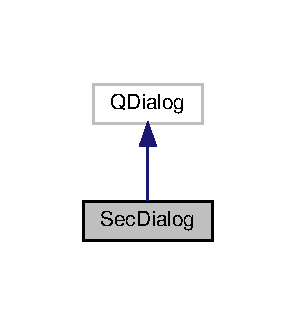
\includegraphics[width=142pt]{classSecDialog__inherit__graph}
\end{center}
\end{figure}


Collaboration diagram for Sec\+Dialog\+:\nopagebreak
\begin{figure}[H]
\begin{center}
\leavevmode
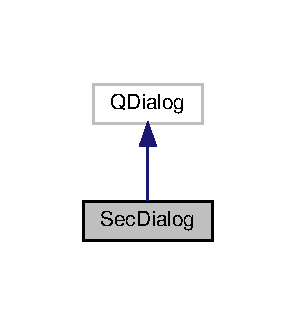
\includegraphics[width=142pt]{classSecDialog__coll__graph}
\end{center}
\end{figure}
\subsection*{Public Member Functions}
\begin{DoxyCompactItemize}
\item 
\mbox{\Hypertarget{classSecDialog_a09f0471b5ec6ac7126a2c65d700ff7b5}\label{classSecDialog_a09f0471b5ec6ac7126a2c65d700ff7b5}} 
{\bfseries Sec\+Dialog} (Q\+Widget $\ast$parent=nullptr)
\end{DoxyCompactItemize}


The documentation for this class was generated from the following files\+:\begin{DoxyCompactItemize}
\item 
src/secdialog.\+h\item 
src/secdialog.\+cpp\end{DoxyCompactItemize}

\hypertarget{classShipment}{}\section{Shipment Class Reference}
\label{classShipment}\index{Shipment@{Shipment}}


The \hyperlink{classShipment}{Shipment} class.  




{\ttfamily \#include $<$Player\+Event.\+h$>$}



Inheritance diagram for Shipment\+:
\nopagebreak
\begin{figure}[H]
\begin{center}
\leavevmode
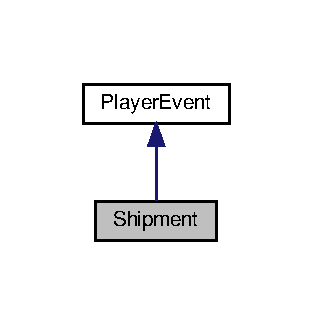
\includegraphics[width=150pt]{classShipment__inherit__graph}
\end{center}
\end{figure}


Collaboration diagram for Shipment\+:
\nopagebreak
\begin{figure}[H]
\begin{center}
\leavevmode
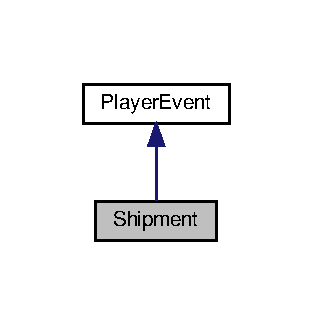
\includegraphics[width=150pt]{classShipment__coll__graph}
\end{center}
\end{figure}
\subsection*{Additional Inherited Members}


\subsection{Detailed Description}
The \hyperlink{classShipment}{Shipment} class. 

The documentation for this class was generated from the following file\+:\begin{DoxyCompactItemize}
\item 
src/Player\+Event.\+h\end{DoxyCompactItemize}

\chapter{File Documentation}
\hypertarget{game_8h}{}\section{src/game.h File Reference}
\label{game_8h}\index{src/game.\+h@{src/game.\+h}}
{\ttfamily \#include $<$string$>$}\newline
{\ttfamily \#include $<$unordered\+\_\+map$>$}\newline
{\ttfamily \#include $<$vector$>$}\newline
{\ttfamily \#include \char`\"{}Player\+Event.\+h\char`\"{}}\newline
{\ttfamily \#include \char`\"{}player.\+h\char`\"{}}\newline
Include dependency graph for game.\+h\+:\nopagebreak
\begin{figure}[H]
\begin{center}
\leavevmode
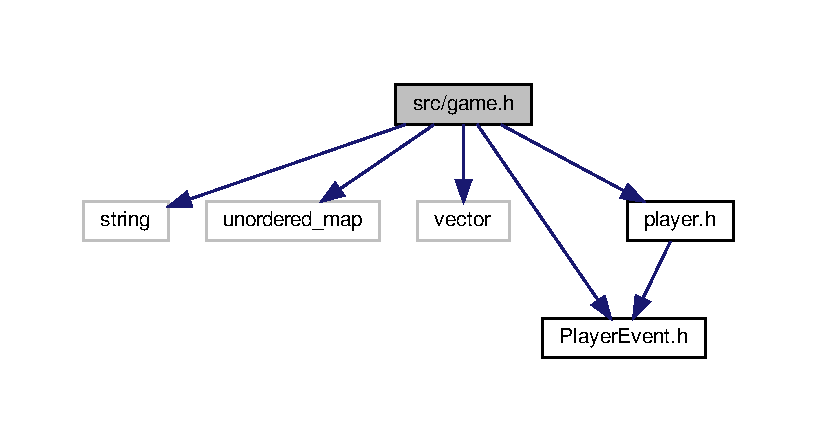
\includegraphics[width=350pt]{game_8h__incl}
\end{center}
\end{figure}
This graph shows which files directly or indirectly include this file\+:\nopagebreak
\begin{figure}[H]
\begin{center}
\leavevmode
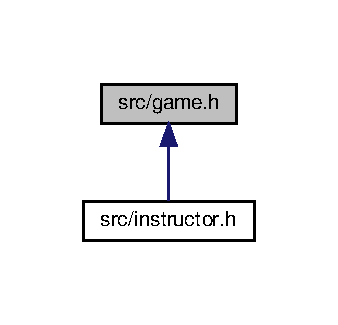
\includegraphics[width=162pt]{game_8h__dep__incl}
\end{center}
\end{figure}
\subsection*{Classes}
\begin{DoxyCompactItemize}
\item 
class \hyperlink{classGame}{Game}
\begin{DoxyCompactList}\small\item\em The \hyperlink{classGame}{Game} class. \end{DoxyCompactList}\end{DoxyCompactItemize}

\hypertarget{instructor_8h}{}\section{src/instructor.h File Reference}
\label{instructor_8h}\index{src/instructor.\+h@{src/instructor.\+h}}
{\ttfamily \#include $<$string$>$}\newline
{\ttfamily \#include $<$vector$>$}\newline
{\ttfamily \#include \char`\"{}game.\+h\char`\"{}}\newline
Include dependency graph for instructor.\+h\+:\nopagebreak
\begin{figure}[H]
\begin{center}
\leavevmode
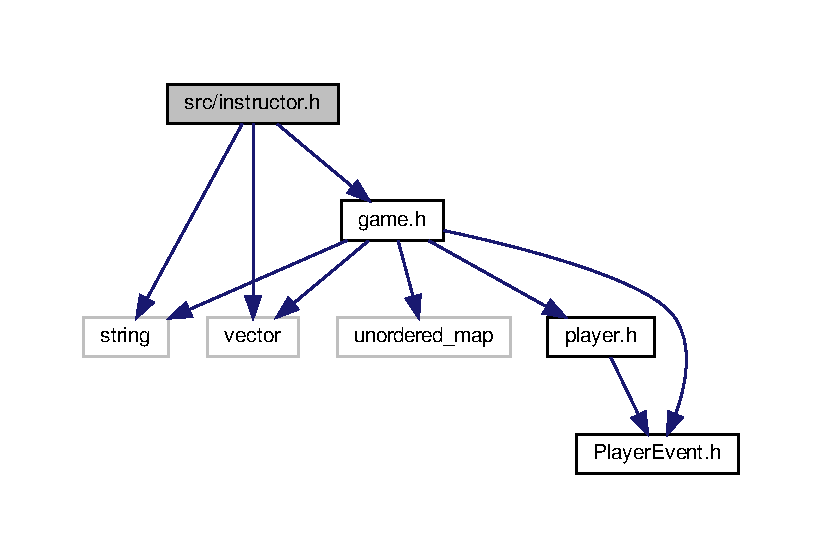
\includegraphics[width=350pt]{instructor_8h__incl}
\end{center}
\end{figure}
\subsection*{Classes}
\begin{DoxyCompactItemize}
\item 
class \hyperlink{classInstructor}{Instructor}
\begin{DoxyCompactList}\small\item\em The \hyperlink{classInstructor}{Instructor} class. \end{DoxyCompactList}\end{DoxyCompactItemize}

\hypertarget{player_8h}{}\doxysection{/home/diggy/sprint-\/1/src/player.h File Reference}
\label{player_8h}\index{/home/diggy/sprint-\/1/src/player.h@{/home/diggy/sprint-\/1/src/player.h}}
{\ttfamily \#include $<$string$>$}\newline
\doxysubsection*{Classes}
\begin{DoxyCompactItemize}
\item 
class \mbox{\hyperlink{class_player}{Player}}
\begin{DoxyCompactList}\small\item\em The \mbox{\hyperlink{class_player}{Player}} class. \end{DoxyCompactList}\end{DoxyCompactItemize}

%--- End generated contents ---

% Index
\backmatter
\newpage
\phantomsection
\clearemptydoublepage
\addcontentsline{toc}{chapter}{Index}
\printindex

\end{document}
